%% Based on a TeXnicCenter-Template by Tino Weinkauf.
%%%%%%%%%%%%%%%%%%%%%%%%%%%%%%%%%%%%%%%%%%%%%%%%%%%%%%%%%%%%%
%%%%%%%%%%%%%%%%%%%%%%%%%%%%%%%%%%%%%%%%%%%%%%%%%%%%%%%%%%%%%
%% HEADER
%%%%%%%%%%%%%%%%%%%%%%%%%%%%%%%%%%%%%%%%%%%%%%%%%%%%%%%%%%%%%
\documentclass{article}

%% Packages for Graphics & Figures %%%%%%%%%%%%%%%%%%%%%%%%%%
\usepackage{graphicx} %%For loading graphic files
%\usepackage{subfig} %%Subfigures inside a figure
%\usepackage{tikz} %%Generate vector graphics from within LaTeX

%% Please note:
%% Images can be included using \includegraphics{filename}
%% resp. using the dialog in the Insert menu.
%% 
%% The mode "LaTeX => PDF" allows the following formats:
%%   .jpg  .png  .pdf  .mps
%% 
%% The modes "LaTeX => DVI", "LaTeX => PS" und "LaTeX => PS => PDF"
%% allow the following formats:
%%   .eps  .ps  .bmp  .pict  .pntg


%% Math Packages %%%%%%%%%%%%%%%%%%%%%%%%%%%%%%%%%%%%%%%%%%%%
\usepackage{amsmath}
\usepackage{amsthm}
\usepackage{amsfonts}
\usepackage{color}
\usepackage{setspace}
\usepackage{listings}
\lstset{language=C++}
\usepackage{lscape} 
\usepackage{float}
\usepackage{graphicx}
\usepackage{caption}
\usepackage{subcaption}
\usepackage[titletoc,toc]{appendix}
%\usepackage{landscape}
\usepackage{xspace}
\usepackage{color}
\textwidth = 450pt
\def\fxnote#1{\marginpar{\textcolor{green}{#1}}}
\def\fxwarning#1{\marginpar{\textcolor{red}{#1}}}
\usepackage[a4paper]{geometry}
\newtheorem{remark}{Remark}[section]
\usepackage{supertabular}
%% Line Spacing %%%%%%%%%%%%%%%%%%%%%%%%%%%%%%%%%%%%%%%%%%%%%
%\usepackage{setspace}
%\singlespacing        %% 1-spacing (default)
%\onehalfspacing       %% 1,5-spacing
%\doublespacing        %% 2-spacing


%% Other Packages %%%%%%%%%%%%%%%%%%%%%%%%%%%%%%%%%%%%%%%%%%%
%\usepackage{a4wide} %%Smaller margins = more text per page.
%\usepackage{fancyhdr} %%Fancy headings
%\usepackage{longtable} %%For tables, that exceed one page


%%%%%%%%%%%%%%%%%%%%%%%%%%%%%%%%%%%%%%%%%%%%%%%%%%%%%%%%%%%%%
%% Remarks
%%%%%%%%%%%%%%%%%%%%%%%%%%%%%%%%%%%%%%%%%%%%%%%%%%%%%%%%%%%%%
%
% TODO:
% 1. Edit the used packages and their options (see above).
% 2. If you want, add a BibTeX-File to the project
%    (e.g., 'literature.bib').
% 3. Happy TeXing!
%
%%%%%%%%%%%%%%%%%%%%%%%%%%%%%%%%%%%%%%%%%%%%%%%%%%%%%%%%%%%%%

%%%%%%%%%%%%%%%%%%%%%%%%%%%%%%%%%%%%%%%%%%%%%%%%%%%%%%%%%%%%%
%% Options / Modifications
%%%%%%%%%%%%%%%%%%%%%%%%%%%%%%%%%%%%%%%%%%%%%%%%%%%%%%%%%%%%%

% common reference commands
\newcommand{\eqt}[1]{Eq.~(\ref{#1})}                     % equation
\newcommand{\fig}[1]{Fig.~\ref{#1}}                      % figure
\newcommand{\tbl}[1]{Table~\ref{#1}}                     % table
\newcommand{\sect}[1]{Section~\ref{#1}}                     % section
\newcommand{\subsect}[1]{Subsection~\ref{#1}}                     % subsection
\newcommand{\app}[1]{Appendix~\ref{#1}}                     % appendix

\newcommand{\ie}{i.e.,\@\xspace}
\newcommand{\eg}{e.g.,\@\xspace}
\newcommand{\psc}[1]{{\sc {#1}}}
\newcommand{\rs}{\psc{R7}\xspace}

\newcommand{\comment}[1]{{\textcolor{red}{#1}}}

%%%%%%%%%%%%%%%%%%%%%%%%%%%%%%%%%%%%%%%%%%%%%%%%%%%%%%%%%%%%%
%% DOCUMENT
%%%%%%%%%%%%%%%%%%%%%%%%%%%%%%%%%%%%%%%%%%%%%%%%%%%%%%%%%%%%%
\doublespacing

\begin{document}

%\pagestyle{empty} %No headings for the first pages.


%% Title Page %%%%%%%%%%%%%%%%%%%%%%%%%%%%%%%%%%%%%%%%%%%%%%%
%% ==> Write your text here or include other files.

%% The simple version:
\title{Numerical solution of the $1$D grey radiation hydrodynamics equations with an entropy-based artificial viscosity.}
\author{Marc-Olivier Delchini\footnote{Nuclear Engineering Department 
Texas A\&M University 3133 TAMU College Station, TX 77843-3133, delchinm@tamu.edu}, Jim Morel\footnote{Nuclear Engineering Department 
Texas A\&M University 3133 TAMU College Station, TX 77843-3133, jim.morel@tamu.edu} and Jean C. Ragusa\footnote{Nuclear Engineering Department 
Texas A\&M University 3133 TAMU College Station, TX 77843-3133, jean.ragusa@tamu.edu }}
%\date{} %%If commented, the current date is used.
\maketitle
\newpage
\addcontentsline{toc}{section}{Abstract}

%%%%%%%%%%%%%%%%%%%%%%%%%%%%%%%%%%%%%%%%%%%%%%%%%%%%%%%%%%%%%
\begin{abstract}
The entropy viscosity method is extended to the 1-D grey radiation-hydrodynamic equations. 
The method employs a viscous regularization to stabilize the numerical scheme with a viscosity coefficient modulated by the entropy production that is known to be peaks in shocks. The dissipative terms are consistent with the entropy minimum principle which requires a new functional form of the entropy residual to be derived, suitable for radiation-hydrodynamic equations. The equations are discretized with a standard Continuous Galerkin Finite Element Method (CGFEM) and implicit temporal integrator within the Moose multiphysics framework. The method of manufactured solution (MMS) is employed to demonstrate second-order accuracy in both the equilibrium diffusion and streaming limits. Several typical 1-D radiation-hydrodynamic test cases with shocks (from Mach 1.05 to Mach 50) are computed to establish the ability of the technique at capturing and resolving shocks.
\end{abstract}
%%%%%%%%%%%%%%%%%%%%%%%%%%%%%%%%%%%%%%%%%%%%%%%%%%%%%%%%%%%%%

\begingroup
    \fontsize{9pt}{9pt}\selectfont
        \smallskip
\noindent \textbf{Keywords:} radiation-hydrodynamics, artificial viscosity, entropy viscosity method.    
\endgroup
\newpage
\marginparwidth = 10pt

%%%%%%%%%%%%%%%%%%%%%%%%%%%%%%%%%%%%%%%%%%%%%%%%%%%%%%%%%%%%%
%%%%%%%%%%%%%%%%%%%%%%%%%%%%%%%%%%%%%%%%%%%%%%%%%%%%%%%%%%%%%
\section{Introduction}
\label{sec:section1}
%%%%%%%%%%%%%%%%%%%%%%%%%%%%%%%%%%%%%%%%%%%%%%%%%%%%%%%%%%%%%
%%%%%%%%%%%%%%%%%%%%%%%%%%%%%%%%%%%%%%%%%%%%%%%%%%%%%%%%%%%%%
Solving the radiation hydrodynamic equations is a challenging task for multiple reasons. First, the characteristic time scales between the radiation and hydrodynamics are different by several orders of magnitude which often requires the radiation part to be solved implicitly to ensure stability. Second, as with any wave-dominated problems, high resolution schemes are needed to accurately resolve shocks. Third, achieving high-order accuracy is challenging but some recent developments provided high-order accuracy results both in time and space when discretized either Euler equations \cite{Hussaini, jlg1, jlg2, Leveque} or the radiation equation independently from each other. \\
%And, fourth, the radiation hydrodynamic equations are stiff to solve in the equilibrium diffusion limit, mainly because of the relaxation source terms that couple the two physics. 
Significant effort has been put into developing Riemann solvers for both the radiation and hydrodynamic equations. Balsara \cite{Balsara} developed a Riemann solver for the radiation-hydrodynamic equations by considering the frozen approximation that decouple the two physics components. However, such an approach can reveal itself questionable in the equilibrium diffusion limit. In this case, the coupling terms drive the physics and have to be accounted for. A \emph{generalized Riemann solver} which accounts exactly for the relaxation terms was developed in \cite{LowrieMorelHittinger}. Another approach, applicable in the equilibrium limit, consists of recasting the system of equations in a conservative form. Then, a numerical solution can be obtained by modifying the equation of state, yielding the radiation-modified equation of state (REOS). This is straightforward to implement in any solver for Euler equations by replacing the equation of state by the REOS \cite{Woodward}. \\
%As mentioned earlier, the high-order accuracy needs to be considered as well. A great amount of work is available in the literature when it comes to solve for Euler equations and the radiation transport equation \cite{Hairer, Wareing}, independent to each other. However, achieving high-order accuracy when coupling the two physics is not an easy process because of the different time scales. 
Edwards and al. proposed a two stage semi-implicit scheme IMEX to solve the coupled radiation-hydrodynamic equations \cite{EdwardsMorelKnoll}. They applied a Trapezoidal/BDF2 temporal discretization scheme to the nonlinear grey radiative diffusion. The radiation and hydrodynamic equations are solved implicitly and explicitly, respectively. A Riemann solver along with a flux limiter is used to resolve shocks and other waves. Their results show good agreement with semi-analytical solutions. \\
In this article we propose to solve the $1$-D radiation-hydrodynamics equations by using \emph{the entropy viscosity method}. This technique, developed by Guermond et al.  for hyperbolic system of equations \cite{jlg1, jlg2}, consists in
adding appropriate dissipative terms to the governing equations  whose viscosity coefficient is modulated by the local entropy production. These dissipative terms are devised so as to stabilize  the numerical scheme and to remove the non-physical oscillations appearing at the shock locations. Generally speaking, entropy is produced at shocks \cite{Toro}. Thus, by setting the viscosity coefficient proportional to the entropy production, shocks can be detected and tracked, and an adequate amount of viscosity is added locally to stabilize the numerical scheme. The entropy production is computed on the fly, by analyzing the entropy residual; this residual is strongly peaked in shocks and small elsewhere. The entropy viscosity method has been shown to achieve high-order accuracy away from the shock regions and
% and first-order convergence in the shock. This method 
was successfully applied to non-linear hyperbolic equation using various discretization methods (finite volume, continuous and discontinuous finite elements, spectral method) and yielded high-order accuracy on non-uniform meshes and complex geometries \cite{jlg2, valentin}. Because of the similarity between Euler equations and the radiation hydrodynamic equations, it is conjectured that the entropy viscosity method may be a good candidate for resolving shocks occurring in radiation-hydrodynamic phenomena.\\
The $1$-D grey radiation-hydrodynamic (GRH) equations are recalled in \eqt{eq:equation1}
and the corresponding variables are defined for clarity purposes:
\begin{equation}
\label{eq:equation1}
\left\{
\begin{array}{lll}
\partial_t \left( \rho \right) + \partial_x\left( \rho u \right) = 0 \\
\partial_t \left( \rho u\right) + \partial_x \left(\rho u^2 + P + \frac{\epsilon}{3} \right) = 0 \\
\partial_t \left( \rho E\right) + \partial_x \left[ u \left( \rho E + P \right) \right] = -\frac{u}{3} \partial_x \epsilon - \sigma_a c \left( a T^4 - \epsilon \right) \\
\partial_t \epsilon + \frac{4}{3} \partial_x \left( u \epsilon \right) = \frac{u}{3} \partial_x \epsilon + \partial_x \left( \frac{c}{3 \sigma_t} \partial_x \epsilon \right) + \sigma_a c \left( a T^4 - \epsilon \right)
\end{array}
\right. ,
\end{equation}
where $\rho$, $u$, $E$, $\epsilon$, $P$ and $T$ are the material density, material velocity, material specific total energy, the radiation energy density, material pressure and temperature, respectively. The total and absorption cross-sections, $\sigma_t$ and $\sigma_a$ are either constant or density- and temperature-dependent. The variables $a$ and $c$ are the Boltzman constant and the speed of light, respectively. Lastly, the symbols $\partial_t$ and $\partial_x$ denote the temporal and spatial partial derivatives, respectively. \
The material temperature and pressure are computed with the Ideal Gas equation of state (IGEOS):
\begin{equation}
\label{eq:equation2}
\left\{
\begin{array}{ll}
P = (\gamma-1) C_v \rho T \\
e = C_v T 
\end{array}
\right.
\end{equation}
where $e$ is the specific internal energy and is obtained from the expression $e = E - 0.5 u^2$. The heat capacity $C_v$ and the heat ratio coefficient $\gamma$ are assumed constant. \\
This paper is organized as follows. In \sect{sec:entropy-visc-meth}, the entropy viscosity method is extended to the grey radiation-hydrodynamic equations;  details regarding the derivation of the adequate dissipative terms and definitions for the new viscosity coefficients are provided. Spatial and temporal discretization schemes are discussed in \sect{sec:num-scheme} along with the solution algorithm employed to solve the discretized equations. Numerical results are presented in \sect{sec:num-res} where second-order accuracy of the scheme is demonstrated in both the equilibrium diffusion and streaming limits, using the method of manufactured solutions applied to the GRH equations. Then, several numerical test cases, taken from the published literature, are provided; in these simulations, the Mach number varies from $1.05$ to $50$ \cite{LowrieEdwards}. Conclusions are presented in \sect{sec:ccl}.

%%%%%%%%%%%%%%%%%%%%%%%%%%%%%%%%%%%%%%%%%%%%%%%%%%%%%%%%%%%%%
%%%%%%%%%%%%%%%%%%%%%%%%%%%%%%%%%%%%%%%%%%%%%%%%%%%%%%%%%%%%%
\section{The entropy-based viscosity method applied to the $1$-D Radiation-Hydrodynamic equations}
\label{sec:entropy-visc-meth}
%%%%%%%%%%%%%%%%%%%%%%%%%%%%%%%%%%%%%%%%%%%%%%%%%%%%%%%%%%%%%
%%%%%%%%%%%%%%%%%%%%%%%%%%%%%%%%%%%%%%%%%%%%%%%%%%%%%%%%%%%%%
In this section, we extend the entropy viscosity method \cite{jlg1, jlg2, valentin} to the $1$-D radiation-hydrodynamic equations in a staged process. First, the reader is guided through the main steps that lead to the derivation of the dissipative terms, using the entropy minimum principle \cite{entropy}. Then, a definition for the entropy viscosity coefficient based upon the entropy production is given. \\
We recall that the entropy viscosity method was developed for hyperbolic system of equations. However, the radiation hydrodynamic equations are not strictly hyperbolic but several numerical techniques are based on the study of their hyperbolic parts \cite{Balsara, LowrieMorel}. Thus, following the same rationale, the system of equations given in \eqt{eq:equation1} is made hyperbolic by assuming an infinite opacity (the frozen approximation) and by ignoring the relaxation terms. These two assumptions yield the following system of equations:
\begin{equation}
\label{eq:equation3}
\left\{
\begin{array}{lll}
\partial_t \left( \rho \right) + \partial_x\left( \rho u \right) = 0 \\
\partial_t \left( \rho u\right) + \partial_x \left(\rho u^2 + P + \frac{\epsilon}{3} \right) = 0 \\
\partial_t \left( \rho E\right) + \partial_x \left[ u \left( \rho E + P \right) \right] = -\frac{u}{3} \partial_x \epsilon\\
\partial_t \epsilon + \frac{4}{3} \partial_x \left( u \epsilon \right) = \frac{u}{3} \partial_x \epsilon
\end{array}
\right. .
\end{equation}
The jacobian matrix of the hyperbolic terms can be computed to derive the eigenvalues:
\begin{equation}
\label{eq:equation4}
\lambda_1 = u-c_m \text{, } \lambda_{2,3} = u \text{ and } \lambda_4 = u+c_m ,
\end{equation}
where $c_m$ is the material speed of sound and is defined as follows:
\begin{equation}
\label{eq:equation5}
c_m^2 = \underbrace{P_{\rho} + \frac{P}{\rho^2}P_e}_{c_{Euler}^2} + \frac{4 \epsilon}{9\rho}
\end{equation}
%\comment{\color{blue}{$P_{\rho}$ has units of $P/\rho$ = units of $e$; $\frac{P}{\rho}P_e $ has units of $P^2/(\rho e)$ = units of $P$ = units of $\rho e$. Something is wrong here. Should the second term be $\frac{P}{\rho^2}P_e $?\\}}
with $P_x$ the standard shorthand notation for $\partial_x P$, and $c^2_{Euler}$ denotes the definition of the speed of sound when only considering the $1$-D Euler equations.
The above hyperbolic system of equations can be recast in a conservative form. This allows us to assume the existence of an entropy function $s$ \cite{Lax} that depends upon the internal energy $e$, the density $\rho$, and the radiation energy density $\epsilon$. Then, following some algebra given in \app{app:appendixA}, an equation satisfied by the entropy $s$ is obtained:
\begin{equation}
\label{eq:equation6}
% D_e(x,t) := 
\rho \frac{ds}{dt} = \rho \left( \partial_t s + u \partial_x s \right) = 0 \text{, }
\end{equation}
where $\frac{d \cdot}{dt}$ denotes the total or material derivative. \eqt{eq:equation6} is often referred as the entropy residual and is used to prove the entropy minimum principle, $\frac{ds}{dt} \geq 0$ \cite{entropy}.\\ When adding dissipative terms to each equation of \eqt{eq:equation3} as required in the entropy viscosity method, the entropy residual equation is modified and some additional terms will appear in the right hand side of \eqt{eq:equation6}. The sign of these extra terms needs to be studied for the entropy minimum principle to hold. As such, the entropy minimum principle is invoked to guide in the derivation of appropriate expressions for each of the dissipative terms. Obtaining the final expression of the dissipative terms is a lengthy process and only the final result along with the key assumptions are stated here. The reader is referred to \app{app:appendixA} for the details of the derivation. The system of equations with the dissipative terms is the following:
\begin{equation}
\label{eq:equation7}
\left\{
\begin{array}{lll}
\partial_t \left( \rho \right) + \partial_x\left( \rho u \right) = \partial_x \left( \kappa \partial_x \rho \right) \\
\partial_t \left( \rho u\right) + \partial_x \left(\rho u^2 + P + \frac{\epsilon}{3} \right) = \partial_x \left( \kappa \partial_x \rho u \right) \\
\partial_t \left( \rho E\right) + \partial_x \left[ u \left( \rho E + P \right) \right] + \frac{u}{3} \partial_x \epsilon = \partial_x \left( \kappa \partial_x(\rho E) \right)\\
\partial_t \epsilon + \frac{4}{3} \partial_x \left( u \epsilon \right) - \frac{u}{3} \partial_x \epsilon = \partial_x \left( \kappa \partial_x \epsilon \right)
\end{array}
\right. ,
\end{equation}
where $\kappa$ is a locally defined positive viscosity coefficient. It was assumed that the following conditions hold:
\begin{equation}
\label{eq:equation7bis}
\left\{
\begin{array}{ll}
P \frac{\partial s}{\partial e} + \rho^2 \frac{\partial s}{\partial \rho} + \frac{4}{3} \rho \epsilon \frac{\partial s}{\partial \epsilon} = 0 \\
s( \rho, e, \epsilon) = \hat{s}(\rho, e) + \frac{\rho_0}{\rho}\tilde{s}(\epsilon) 
\end{array}
\right.
\end{equation}
where $-\tilde{s}$ is convex with respect to the radiation energy density $\epsilon$ and $-\hat{s}$ is convex with respect to the internal energy $e$ and the specific volume $\frac{1}{\rho}$. The constant $\rho_0$ is of order one and appears only for dimensionality purposes. \\
Once the dissipative terms are obtained, it remains to define the local viscosity coefficient $\kappa(x,t)$. 
%This is not an easy task and great care needs to be taken. It is proposed to explain the reasoning that leads to a definition for the viscosity coefficient $\kappa$. The definition of the viscosity coefficient $\kappa$ must meet the three following requirements:
We require the following to hold in the prescription for $\kappa$:
\begin{itemize}
\item An upper bound on $\kappa$ is required for stability of the numerical scheme: when considering explicit temporal integrators, the maximum value of the viscosity coefficient is related to the Courant-Friedrichs-Lewy number (CFL). This upper bound is defined by analogy to the standard upwind (Godunov) scheme that is known to efficiently smooth out oscillations (but is only first-order accurate). With implicit temporal integrators, the same reasoning is used even if the CFL number is, in theory, no longer required. This upper bound will be referred to as the \emph{first-order viscosity}, denoted by $\kappa_{max}(x,t)$.  
\item Since the entropy residual is a measure of the entropy production that occurs in shock regions, it is natural to define a viscosity coefficient proportional to the entropy residual. This will enable shock detection and tracking and will also provide a measure of the viscosity required to stabilize the scheme. This viscosity coefficient is referred to as the \emph{entropy viscosity coefficient} or \emph{second-order viscosity coefficient} and is denoted by $\kappa_e(x,t)$.
\item The viscosity coefficient that is actually used in the dissipative terms, $\kappa$, of \eqt{eq:equation3} is defined as follows: $\kappa(x,t) = \min ( \kappa_e(x,t), \kappa_{max}(x,t) )$. With such a definition, the viscosity added to the system of equation will saturate to the first order viscosity in the shock regions. Elsewhere, the entropy production and the viscosity coefficient $\kappa$ are expected to be small.
\end{itemize}
Next, we define the first- and second-order viscosity coefficients. Following the work of Zingan et al. \cite{valentin}, the first-order viscosity definition is based on the local largest eigenvalue that is known to be $|u| + c_m$ in $1$-D:
\begin{equation}
\label{eq:equation8}
\kappa_{max} = \frac{h}{2} \left( |u| + c_m \right)
\end{equation}  
where $h$ is the local grid size. This definition is derived based on the upwind scheme and a simple derivation can be found in \cite{jlg1} in the case of a scalar hyperbolic equation. Through the definition of the speed of sound $c_m$, both the material and radiation properties are accounted for in the definition of the first-order viscosity coefficient.\\
The definition of the second order viscosity coefficient, $\kappa_e(x,t)$, is based upon the entropy residual (\eqt{eq:equation6}) that can be recast as a function of pressure $P$, density $\rho$ and radiation energy density $\epsilon$:
% (\app{app:appendixA}):
\begin{equation}
\label{eq:equation9}
%\tilde{D}_e(x,t) = \frac{s_e}{P_e} \underbrace{ \left( \frac{dP}{dt} - c_m^2 \frac{d\rho}{dt} + \frac{d\epsilon}{dt} \right)}_\textrm{$\hat{D}_e(x,t)$}
\tilde{D}_e(x,t) = \frac{s_e}{P_e} \underbrace{ \left( \frac{dP}{dt} - c_{Euler}^2 \frac{d\rho}{dt} \right)}_\textrm{$\hat{D}_e(x,t)$}
\end{equation}
%\comment{\color{blue}{the reader will not be able to see the connection with the appendix because in the appendix there are no such equations as Eq.(10). If you recall in the main text a result from the appendix, it should be found in the appendix\\}}
The term $s_e$ is the inverse of the material temperature (\app{app:appendixA}) and $P_e$ is computed from the IGEOS. These two terms are positive so that the sign of the entropy residual $\tilde{D}_e(x,t)$ can be determined by simply inspecting the terms inside the parentheses, denoted by $\hat{D}_e(x,t)$. Such an expression is easier to compute than the one given in \eqt{eq:equation6} which required an analytical expression for the entropy function. In addition to the entropy residual, inter-element jumps in the pressure and density gradients, $J$, are also accounted for. The objective is to be able to also detect discontinuities that are not shocks, such as contact waves (there is no entropy production in a contact wave), in order to stabilize them as well. \\
Thus, the entropy viscosity coefficient $\kappa_e(x,t)$ is set to be proportional to $\hat{D}_e(x,t)$ and $J$ with the following form: 
\begin{equation}
\label{eq:equation12}
\kappa_e(x,t) = h^2 \frac{\max (|\hat{D}_e(x,t)|, J)}{n_P}
\end{equation} 
where $J = \max_i (J(x_i,t))$, and $J(x_i,t)$ is the jump of a given quantity at cell interface $x_i$, and $n_P$ is a normalization function (of the same unit as pressure) that has to be chosen so that the viscosity coefficient $\kappa$ is of unit $m^2/s$. It is chosen to take the following definition for the normalization function: $n_P = \rho c_m^2$. Thus, the final definition for the viscosity coefficient $\kappa$ is the following:
\begin{equation}
\label{eq:equation12bis}
\kappa_e(x,t) = h^2 \frac{\max (|\hat{D}_e(x,t)|, J)}{\rho c_m^2}
\end{equation} 
The jump $J$ in the definition of $\kappa(x,t)$ is piecewise-constant. Its definition is discretization-dependent and defined as follows for Continuous Galerkin FEM: 
\begin{equation}
\label{eq:equation12ter}
\left\{
\begin{array}{lll}
J_P(x_i,t) = |u| [[\partial_x P]]\\
J_{\rho}(x_i,t) = c_m^2 |u|  [[\partial_x \rho]] \\
J(x_i,t) = \max( J_{\rho}(x_i,t), J_{P}(x_i,t) )
\end{array}
\right.
\end{equation}
%The jumps of the pressure and density gradient are included in the definition of the viscosity coefficients since they are a good shock indicator (with CGFEM, the variables are continuous at the interface but their gradients are discontinuous). 
The symbol $[[ \cdot ]]$ denotes the jump at the interface.\\
%The reader will notice that the pressure jump is proportional to $(|u|+c_m)$ since the pressure varies in the shock. On another hand, the density jump is proportional to the material velocity that is the eigenvalue associated to the contact wave. \\
The entropy viscosity method is now well defined for the hyperbolic system given in \eqt{eq:equation3} and will be used to solve for the grey radiation-hydrodynamic equations given in \eqt{eq:equation1}. However, one may question how the relaxation source terms, $\sigma_a c (a T^4-\epsilon)$ and the physical diffusion term, $\partial_x(D\partial_x \epsilon)$, may affect the entropy viscosity method. When applying the entropy viscosity method, the radiation energy density equation will now contain a diffusive term and a numerical dissipative term with a vanishing viscosity coefficient $\kappa$. As long as the diffusive coefficient $D=\frac{c}{3 \sigma_t}$ is larger than the viscosity coefficient $\kappa$, the numerical dissipative term should not be required. A way to ensure consistency and prevent the formation of oscillations in the frozen limit is to merge the two second-order derivative terms into one as follows:
 \begin{equation}
 \partial_x \left( \frac{c}{3 \sigma_t} \partial_x \epsilon \right) + \partial_x \left( \kappa \partial_x \epsilon \right) = \partial_x \left[ \max\left(\frac{c}{3 \sigma_t} \text{, } \kappa \right) \partial_x \epsilon \right]
 \end{equation}
 Thus, as long as the artificial viscosity coefficient $\kappa$ is locally smaller that the physical diffusive coefficient $D=\frac{c}{3 \sigma_t}$, no artificial viscosity is required to ensure stability of the numerical scheme. As the diffusive coefficient $D$ goes to zero, shocks can form in the radiation energy density profile and will require a certain amount of viscosity in order to prevent oscillations from appearing. \\
The effect of the relaxation source terms onto the entropy viscosity method can become problematic in the equilibrium diffusion limit $(\sigma_a c \to \infty)$: the relaxation source terms behave as dissipative terms and make the system parabolic \cite{Leveque}. In \cite{ShiJin}, a study on the impact of various artificial viscosity methods onto hyperbolic systems with relaxation terms was carried out. It was shown that high-order viscosity coefficients are better suitable since they do not alter the physical solution as much as first-order viscosity such as the upwind scheme. A manufactured method solution is designed in \sect{sec:MMS} to test the convergence of the numerical solution in the equilibrium-diffusion limit.  
\begin{remark}
The normalization factor has to be larger than $h$ in order to conserve the high-order accuracy.%\comment{can you prove or provide evidence for this? \color{blue}{we need to talk about it}}
 \end{remark}
 \begin{remark}
The reader will notice that, except for the definition of the jumps, the whole method is independent of the spatial discretization employed. The technique could be used with discontinuous Galerkin finite element or finite volume methods. In both cases, an adequate  definition of the jump terms can be found in \cite{valentin}.
 \end{remark}

%%%%%%%%%%%%%%%%%%%%%%%%%%%%%%%%%%%%%%%%%%%%%%%%%%%%%%%%%%%%%
%%%%%%%%%%%%%%%%%%%%%%%%%%%%%%%%%%%%%%%%%%%%%%%%%%%%%%%%%%%%%
\section{Numerical scheme and solution technique}
\label{sec:num-scheme}
%%%%%%%%%%%%%%%%%%%%%%%%%%%%%%%%%%%%%%%%%%%%%%%%%%%%%%%%%%%%%
%%%%%%%%%%%%%%%%%%%%%%%%%%%%%%%%%%%%%%%%%%%%%%%%%%%%%%%%%%%%%
The 1-D radiation-hydrodynamic equations \eqt{eq:equation1} are discretized with the continuous Galerkin finite element method (CGFEM) under the Moose framework \cite{Moose}. \\ 
%The Moose framework makes available to us a wide range of test functions and quadrature rules. \\
To obtain a weak form, the following generic form of \eqt{eq:equation1} is considered:
\begin{equation}
\label{eq:form}
\partial_t U + \partial_x F \left( U \right) = S + \partial_x H \left(U\right)
\end{equation}
where $U$ is the vector solution, $F$ is a conservative vector flux, $S$ is a vector containing the relaxation source terms and non-conservative terms, and $H$ is the artificial viscosity dissipative flux:
\begin{eqnarray}
U = \left[
\begin{array}{cccc}
\rho \\
\rho u \\
\rho E \\
\epsilon
\end{array}
\right], \text{ }
F(U) = \left[
\begin{array}{cccc}
\rho u \\
\rho u^2 + P + \frac{\epsilon}{3} \\
u \left( \rho E + P \right) \\
\frac{4}{3} u \epsilon
\end{array} 
\right] \text{, } \nonumber \\
S = \left[
\begin{array}{cccc}
0 \\
0 \\
-\frac{u}{3} \partial_x \epsilon - \sigma_a c \left( a T^4 - \epsilon \right) \\
\frac{u}{3} \partial_x \epsilon + \partial_x \left( \frac{c}{3 \sigma_t} \partial_x \epsilon \right) + \sigma_a c \left( a T^4 - \epsilon \right)
\end{array}
\right] \text{ and } \nonumber \\ 
H(U) = \left[
\begin{array}{cccc}
\kappa \partial_x \rho \\
\kappa \partial_x (\rho u) \\
\kappa \partial_x \left( \rho e \right) + \frac{u^2}{2} \kappa \partial_x \rho + \rho u \mu \partial_x u
\end{array}
\right]
\nonumber
\end{eqnarray}
In order to apply the continuous finite element method, \eqt{eq:form} is multiplied by a smooth test function $\phi$, integrated by parts over each finite element $e$ of the discrete mesh $\Omega$ bounded by $\partial \Omega$, to obtain a weak solution:
\begin{eqnarray}
\sum_e \int_{e} \partial_t U \phi - \sum_e \int_{e} F(U) \partial_x \phi + \int_{\partial \Omega} F(U) \mathbf{n} \phi - \nonumber\\ \sum_e \int_{e} S \phi + \sum_e \int_{e} H(U) \partial_x \phi - \int_{\partial \Omega}H \left( U \right) \mathbf{n} \phi= 0
\end{eqnarray}
where $\mathbf{n}$ is the outward normal vector to the boundary of the computational domain. \\
The integrals over the elements $e$ are evaluated using either trapezoidal or Gauss quadrature rules. The time-dependent term will be evaluated using the implicit second-order temporal integrator BDF2 \cite{Leveque}. Only linear polynomials test functions are considered in this paper.\\
The integral on $\partial \Omega$ requires computation of the flux $F(U)$ and $H(U)$ on the boundary. It is chosen to treat the boundary for each physics component independently and details will be given in \sect{sec:simulations} on how to compute $F(U)$. The viscosity dissipative flux $H(U)$ is zero on the boundaries since the viscosity coefficients $\kappa$ and $\mu$ are set to zero \cite{jlg1, jlg2, valentin}. \\
The Jacobian-Free Newton Krylov method \cite{JFNK} is employed to solve the system for each time step: Newton's and Krylov methods are used for the outer nonlinear and inner linear solves, respectively. The full Jacobian matrix is used as a preconditioner and is computed by finite difference: this options is available in Moose and remains efficient for 1-D simulations. 
 \begin{remark}
The entropy residual expression is not integrated over the cell volume as it is usually done in the Galerkin finite element method. The variable values and their gradients are available at quadrature points and at different times, and, thus, can be used to evaluate the entropy residual. 
%The time-derivative term is discretized with the second-order temporal integrator, BDF2 \cite{Leveque}. 
\end{remark}
%\comment{\color{blue}{This section does not need to be too long but I feel like stating the temporal scheme, giving the weak CGFEM form, and mentioning PJFNK, all of which you do in the Numerical results sections, would be better done here, in a separate section. This would also give more chances to the reader to understand how you discretize and solve the system of equations}}
%%%%%%%%%%%%%%%%%%%%%%%%%%%%%%%%%%%%%%%%%%%%%%%%%%%%%%%%%%%%%
%%%%%%%%%%%%%%%%%%%%%%%%%%%%%%%%%%%%%%%%%%%%%%%%%%%%%%%%%%%%%
\section{Numerical results}
\label{sec:num-res}
%%%%%%%%%%%%%%%%%%%%%%%%%%%%%%%%%%%%%%%%%%%%%%%%%%%%%%%%%%%%%
%%%%%%%%%%%%%%%%%%%%%%%%%%%%%%%%%%%%%%%%%%%%%%%%%%%%%%%%%%%%%

In this section, numerical results of the dimensional $1$D grey radiation-hydrodynamic equations are presented using the entropy viscosity method. First, second-order accuracy of the method is demonstrated using the method of manufactured solution (MMS). Then, some typical test cases for radiation-hydrodynamic equations are given. 
%The equations are discretized using CGFEM in the Moose framework \cite{Moose}. First order polynomials are used for the spatial discretization. The second-order BDF2 implicit temporal integrator is employed. The system is solved by a Preconditioned Jacobian Free Newton Krylov solver (PJFNK) where the full jacobian matrix is used as a preconditioner. 

%%%%%%%%%%%%%%%%%%%%%%%%%%%%%%%%%%%%%%%%%%%%%%%%%%%%%%%%%%%%%
\subsection{Space/time accuracy}
\label{sec:MMS}
%%%%%%%%%%%%%%%%%%%%%%%%%%%%%%%%%%%%%%%%%%%%%%%%%%%%%%%%%%%%%

The same manufactured solution as in \cite{EdwardsMorelLowrie} is used in order to test both the diffusive and streaming limit solutions in a slab of thickness $L=2 \pi$ $cm$. The manufactured solutions are composed of trigonometric functions. Periodic boundary conditions are used for all of the variables. The L$_2$ norm errors between the numerical and exact solutions are computed for density, momentum, total material energy, and radiation energy density. For each new simulation, the time step is divided by two and the  number of spatial degrees of freedom is doubled. With such settings, the error is expected to decrease by a factor $4$ if second-order convergence is achieved. \\
The first manufactured solution is designed to test the equilibrium-diffusion limit. In that case, the radiation energy is in equilibrium with the material temperature and the opacity is large which means that the radiation mean-free path is not resolved. The following exact solution was used:
\begin{equation}
\label{eq:equation13}
\left\{
\begin{array}{llll}
\rho = \sin (x-t)+2 \\
u = \cos(x-t) +2 \\
T = \frac{0.5 \gamma (\cos(x-t) +2) }{\sin (x-t)+2}\\
\epsilon = a T^4
\end{array}
\right.
\end{equation}
The cross sections $\sigma_a$ and $\sigma_t$ are assumed constant and set to the same value $1000$ $cm^{-1}$. The simulation is run until $t=3$ $sh$. The L$_2$ error norm along with the ratio between consecutive simulations are given in \tbl{tbl:table1} for the equilibrium diffusion limit:
\begin{table}[H]
\caption{\label{tbl:table1} Convergence study for the first manufactured solution.}
\begin{center}
\begin{tabular}{|c|c|c|c|c|c|c|c|c|c|}
\hline
\textbf{DoF} & $\mathbf{\Delta t}$ $\mathbf{(sh)}$  & $\mathbf{\rho}$ & \textbf{ratio} & $\mathbf{\rho E}$ & \textbf{ratio} \\ \hline
$20$ & $10^{-1}$ &	 $0.590766$ & NA &  $1.333774$ & NA \\ \hline
$40$ & $5$ $10^{-1}$ & $0.290626$ & $2.03$ &  $0.478819$ & $2.79$ \\ \hline
$80$ & $2.5$ $10^{-2}$ & $0.0959801$ & $3.021$ &  $0.154119$ & $3.11$ \\ \hline
$160$ & $1.25$ $10^{-2}$ & $0.02593738$ & $3.70$ &  $0.0405175$ & $3.80$ \\ \hline
$320$ & $6.25$ $10^{-3}$ & $6.471444$ $10^{-3}$ & $4.00$ & $9.90446$ $10^{-3}$ & $4.09$ \\ \hline
$640$ & $3.125$ $10^{-3}$ & $1.584158$ $10^{-3}$ & $4.01$ & $2.44727$ $10^{-3}$ & $4.04$ \\ \hline
\hline
\textbf{DoF} & $\mathbf{\Delta t}$ $\mathbf{(sh)}$ & $\mathbf{\epsilon}$ & \textbf{ratio} &  $\mathbf{\rho u}$ & \textbf{ratio} \\ \hline
$20$ & $10^{-1}$ &  $0.00650085$ & NA & $0.910998$ & NA	\\ \hline
$40$ & $5$ $10^{-1}$ &  $0.00124983$ & $5.20$ & $0.4090946$ & $2.23$	\\ \hline
$80$ & $2.5$ $10^{-2}$ &  $0.000262797$ & $4.76$ & $0.125943$ & $3.25$	\\ \hline
$160$ & $1.25$ $10^{-2}$ &  $6.17726$ $10^{-5}$ & $4.25$ & $3.381042$ $10^{-3}$ & $3.72$	\\  \hline
$320$ & $6.25$ $10^{-3}$ & $1.509184$ $10^{-5}$ & $4.09$ & $8.373657$ $10^{-3}$ & $4.04$ \\ \hline 
$640$ & $3.125$ $10^{-3}$  & $3.72548$ $10^{-6}$ & $4.05$ & $2.070538$ $10^{-3}$ & $4.04$ \\ \hline   
\end{tabular}  
\end{center}
\end{table}
The second manufactured solution is used to test the streaming limit: the radiation streaming dominates the absorption/re-emission term and evolves at a fast time scale. The exact solutions are the following:
\begin{equation}
\label{eq:equation14}
\left\{
\begin{array}{llll}
\rho = \sin(x-t)+2 \\
u = \left( \sin(x-t)+2 \right)^{-1} \\
T = 0.5 \gamma \\
\epsilon = \sin(x-1000 t)+2
\end{array}
\right.
\end{equation}
For this manufactured solution, the cross sections are still assumed constant and set to the same value $1$ $cm^{-1}$. The final time is $t_{final}=3.$ $sh$. 
Once again, the L$_2$ error is given in \tbl{tbl:table2} for the density, momentum, material total energy and radiation energy density.
\begin{table}[H]
\begin{center}
\caption{\label{tbl:table2} Convergence study for the second manufactured solution.}
\begin{tabular}{|c|c|c|c|c|c|}
\hline
\textbf{DoF} & $\mathbf{\Delta t}$ $\mathbf{(sh)}$  & $\mathbf{\rho}$ & \textbf{ratio} & $\mathbf{\rho E}$ & \textbf{ratio} \\ \hline
$20$ &$10^{-1}$& $1.4373$ $10^{-2}$ & NA & $5.88521$ $10^{-1}$ & NA \\ \hline
$40$ & $5.$ $10^{-2}$& $3.760208$ $10^{-3}$ & $3.82$ & $1.4244$ $10^{-1}$ & $4.13$ \\ \hline 
$80$ & $2.5$ $10^{-2}$& $9.91724$ $10^{-4}$ & $3.79$ & $3.2047$ $10^{-2}$ & $4.44$  \\ \hline      
$160$ & $1.25$ $10^{-2}$ & $2.4455$ $10^{-4}$ & $4.06$ & $7.4886$ $10^{-3}$ & $4.28$  \\ \hline     
$320$ & $6.25$ $10^{-3}$ & $6.280715$ $10^{-5}$ & $3.89$ & $1.82327$ $10^{-3}$ & $4.11$ \\ \hline 
$640$ & $3.125$ $10^{-3}$ & $1.57920$ $10^{-5}$ & $3.98$ & $4.50463$ $10^{-4}$ & $4.05$  \\ \hline
$1280$ & $1.5625$ $10^{-4}$ & $3.96096$ $10^{-6}$ & $3.99$ & $1.12061$ $10^{-4}$ & $4.02$ \\ \hline
\hline
\textbf{DoF} & $\mathbf{\Delta t}$ $\mathbf{(sh)}$ & $\mathbf{\epsilon}$ & \textbf{ratio} &  $\mathbf{\rho u}$ & \textbf{ratio} \\ \hline
$20$ &$10^{-1}$ & $3.82001$ $10^{-1}$ & NA & $2.354671$ $10^{-3}$ & NA \\ \hline
$40$ & $5.$ $10^{-2}$ & $1.21500$ $10^{-1}$ &$3.14$& $6.138814$ $10^{-4}$& $3.84$ \\ \hline
$80$ & $2.5$ $10^{-2}$ & $3.27966$ $10^{-2}$ &$3.70$& $1.74974$ $10^{-4}$ & $3.51$ \\ \hline
$160$ & $1.25$ $10^{-2}$ & $8.38153$ $10^{-3}$ &$3.91$& $3.61297$ $10^{-5}$  & $4.84$ \\ \hline
$320$ & $6.25$ $10^{-3}$ & $2.10925$ $10^{-3}$ &$3.97$& $9.03866$ $10^{-6}$ & $3.99$ \\ \hline
$640$ & $3.125$ $10^{-3}$ & $5.28472$ $10^{-4}$ &$3.99$& $2.25649$ $10^{-6}$ & $4.01$ \\ \hline
$1280$ & $1.5625$ $10^{-4}$ &$1.322268$ $10^{-4}$ &$3.99$& $5.69984$ $10^{-7}$ & $3.95$ \\ \hline
\end{tabular}
\end{center}
\end{table}
For both manufactured solutions the error is divided by four as the time step $\Delta t$ and the spatial mesh $\Delta x$ are reduced by a factor two. Thus, we conclude that the entropy viscosity method allows the scheme to be second-order accurate when the numerical solution is smooth. 
%\comment{Expect for a quick look at the appendix, I have stopped here and will resume for this point onward soon \color{blue}{ok}}

%%%%%%%%%%%%%%%%%%%%%%%%%%%%%%%%%%%%%%%%%%%%%%%%%%%%%%%%%%%%%
\subsection{Radiation shock simulations}
%%%%%%%%%%%%%%%%%%%%%%%%%%%%%%%%%%%%%%%%%%%%%%%%%%%%%%%%%%%%%
\label{sec:simulations}
The purpose of this section is to show that the entropy-based viscosity method (\sect{sec:entropy-visc-meth}) can resolve shocks occuring in radiation-hydrodynamic simulations. Multiple test cases are considered with Mach numbers of $1.05$, $1.2$, $2$, $5$ and $50$ \cite{LowrieEdwards}. All of the simulations are run with $500$ cells and with a Courant-Friedrichs-Lewy (CFL number) of $10$ until steady-state (even if the scheme employed here is fully implicit, a CFL number can still be computed and is a good reference for comparison against semi-implicit or fully explicit codes). Linear Lagrange polynomials and the second-order temporal integrator BDF2 are once again used. For clarity, the initial conditions of each test case will be given in a table and plots of the density ($\rho (x)$), the radiation ($\theta (x)$) and material ($T(x)$) temperatures at steady-state will be shown as well as the local viscosity coefficients $\kappa(x)$ and $\kappa_{max}(x)$. The computational domain consists of a $1$D slab of thickness $L$. The initial step is located at $x_0$ and will be specified for all of test cases. For all of the test cases presented in this paper the cross sections $\sigma_a$ and $\sigma_t$ are assumed constant and set to $853.144$ $cm^{-1}$ and $390.711$ $cm^{-1}$, respectively, if not otherwise specified. The heat capacity at constant specific volume is set to $C_v = 0.12348$ $jerks/(g-keV)$.\\
For the Mach $2$ simulation, results will be shown when employing the first-order viscosity $(\kappa(x,t) = \kappa_{max}(x,t))$. The rational for this is to show the benefits of using a high-order viscosity coefficients. \\
The inlet and outlet BCs are given next. The Euler equations and radiation equation are considered independently since the later one is parabolic. At the inlet, the flow is supersonic and, therefore, no physical information exits the system. Thus, Dirichlet boundary condition can be used. At the outlet, the flow become subsonic which requires a particular treatment. Following the work from \cite{SEM}, a static boundary condition is implemented. Only the back pressure is provided and the other variables are computed using the characteristic equations. For the radiation equation, vacuum boundary conditions are used at both inlet and outlet.

\subsubsection{An equilibrium diffusion test:}
%%%%%%%%%%%%%%%%%%%%%%%%%%%%%%%%%%%%%%%%%%%%%%%%%%%%%%%%%%%%%

For this test, the inlet Mach number is set to $1.05$. The radiation field and material are in equilibrium. The initial conditions are given in \tbl{tbl:table3}.
\begin{table}[h]
\begin{center}
\caption{\label{tbl:table3} Initial conditions for Mach $1.05$.}
\begin{tabular}{|c|c|c|}
\hline 
 & left  & right \\ \hline
$\rho$ $(g/cm^3)$ &$1.$ & $1.0749588$ \\ \hline
$u$ $(cm/sh)$& $0.1228902$ & $0.1144127$ \\ \hline
$T$ $(keV)$& $0.1$ & $0.1049454$\\ \hline
$\epsilon$ $(jerks/cm^3)$ & $1.372$ $10^{-6}$ & $1.6642117$ $10^{-6}$\\
\hline
\end{tabular}
\end{center}  
\end{table}  
The computational domain is of size $L=0.030$ $cm$ and the initial step was located in the middle at $x_0 = 0.015$ $cm$. The numerical solutions at steady-state are given in \fig{fig:Mach105_temp}, \fig{fig:Mach105_density} and \fig{fig:Mach105_viscosity}. The solution was run with $CFL = 10$.
\begin{figure}[H]
                \centering
                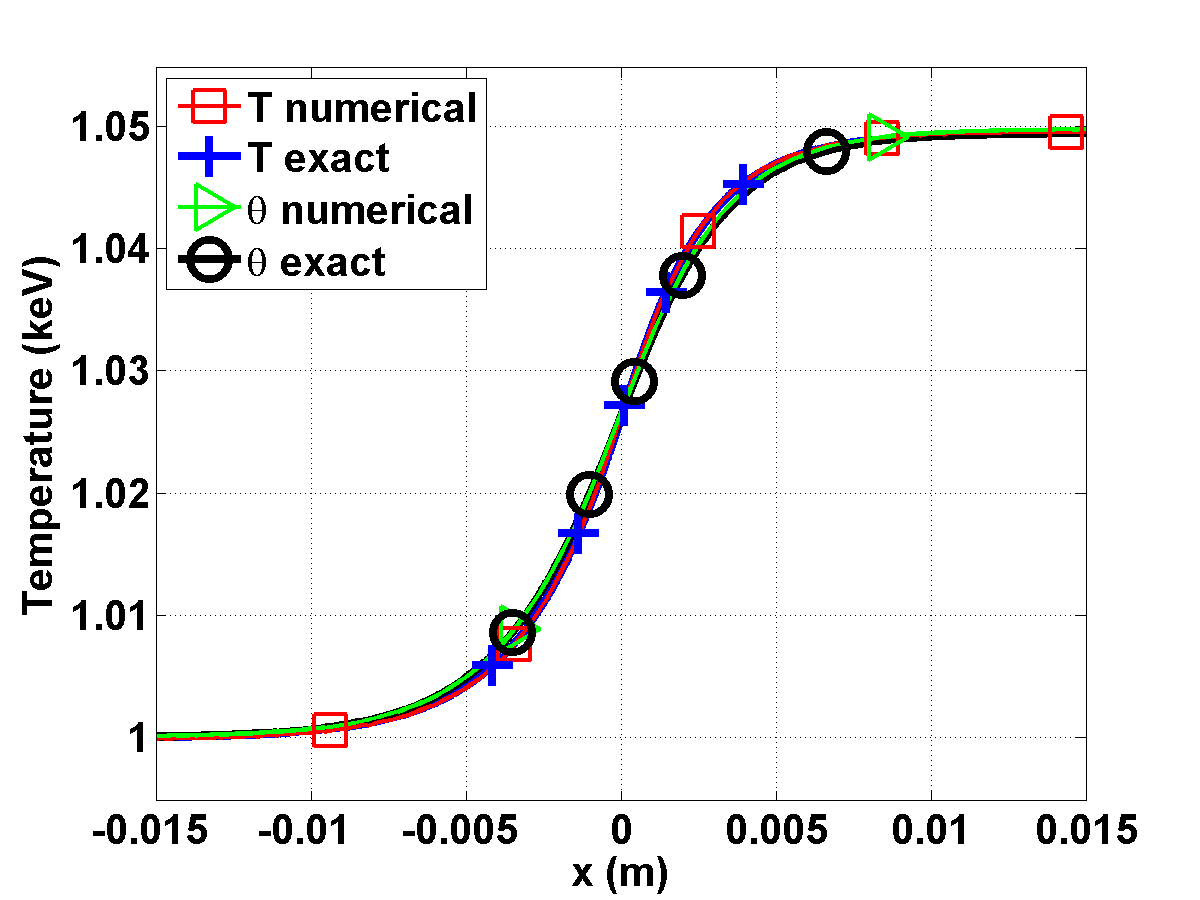
\includegraphics[width=\textwidth]{Mach_1p05_nel_500_temperature.png}
        \caption{Material and radiation temperature profiles at steady-state for Mach 1.05 test.}\label{fig:Mach105_temp}
\end{figure}
\begin{figure}[H]
                \centering
                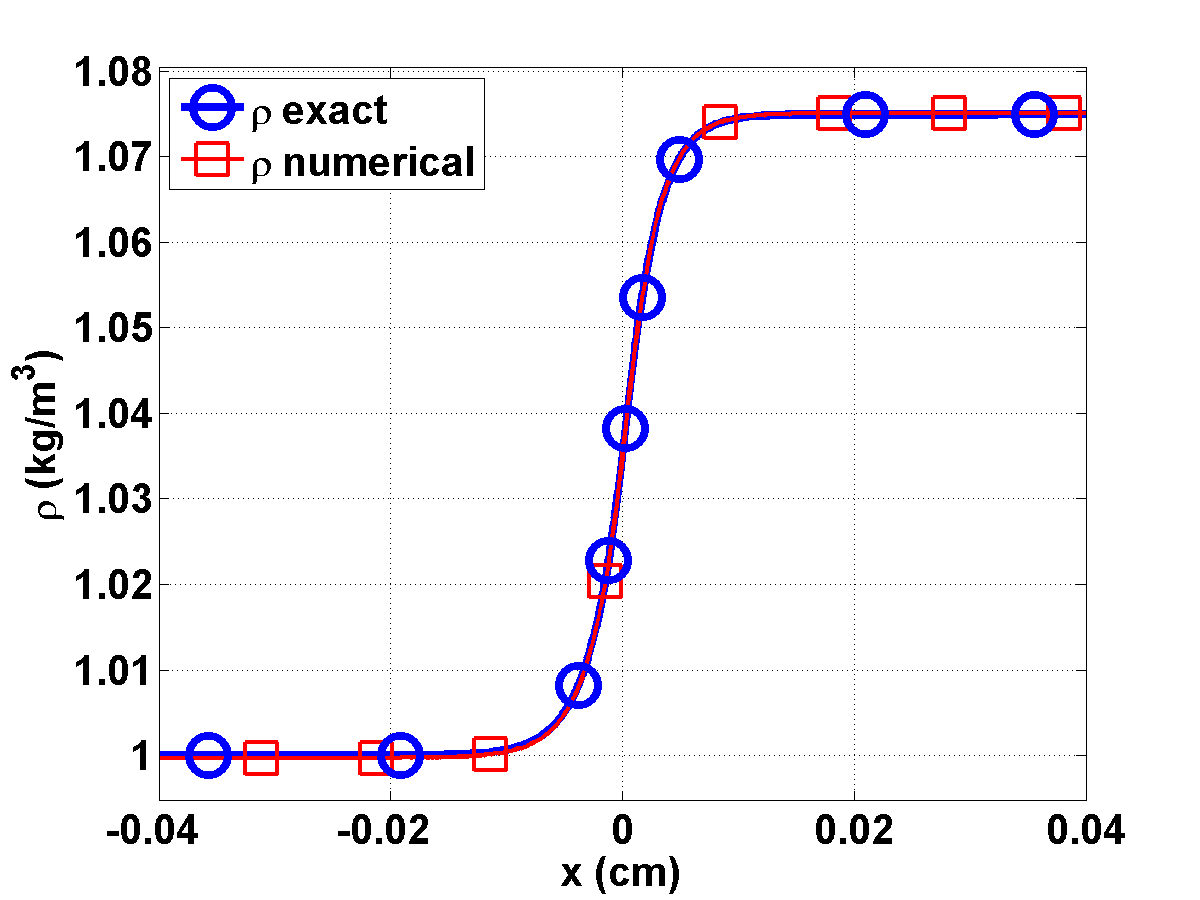
\includegraphics[width=\textwidth]{Mach_1p05_nel_500_density}
        \caption{Material density profile at steady-state for Mach 1.05 test.}\label{fig:Mach105_density}
\end{figure}
\begin{figure}[H]
                \centering
                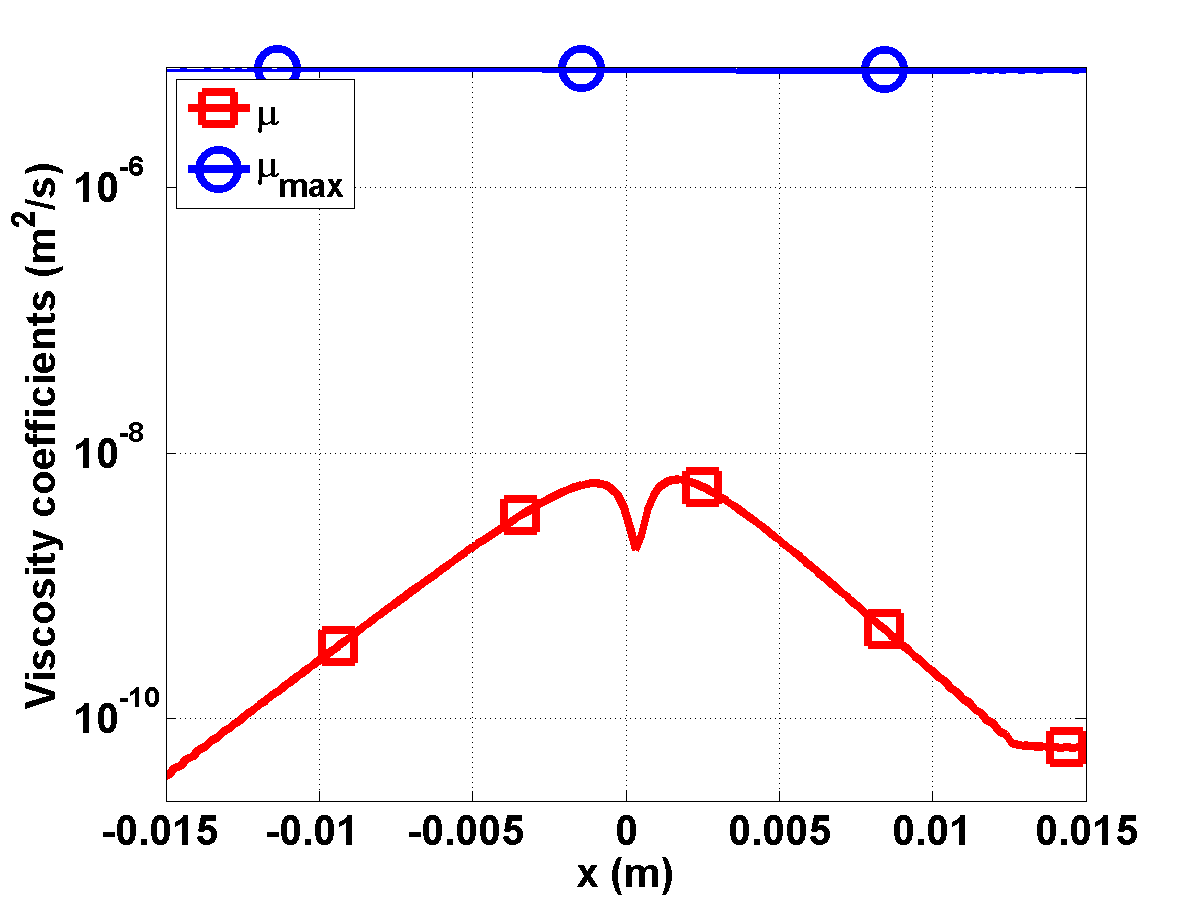
\includegraphics[width=\textwidth]{Mach_1p05_nel_500_viscosity.png}
        \caption{First-order viscosity $\kappa_{max}$ and second-order viscosity $\kappa$ profiles at steady-state for Mach 1.05 test (logarithm scale).}\label{fig:Mach105_viscosity}
\end{figure}
The energy transfer between the material and radiation fields is not large enough to form a shock in the material. Thus, all of the material variables are smooth (\fig{fig:Mach105_temp} and \fig{fig:Mach105_density}) as well as the radiation temperature $\theta$. Because of the smoothness of the solution, the viscosity coefficient $\kappa$ is three order of magnitude smaller than the first-order viscosity coefficient $\kappa_{max}$ (\fig{fig:Mach105_viscosity}): in other words, the viscosity added to the system is large enough to stabilize it, but sufficiently small so that the physical solution is not disturbed.

\subsubsection{A $1.2$ Mach hydrodynamic shock:}
%%%%%%%%%%%%%%%%%%%%%%%%%%%%%%%%%%%%%%%%%%%%%%%%%%%%%%%%%%%%%

In this test, the material experiences a shock and the radiation energy density remains smooth. The initial conditions, corresponding to a Mach number of $1.2$ at the inlet, are as follows: 
\begin{table}[H]
\caption{\label{tbl:table4} Initial conditions for Mach $1.2$.}
\begin{center}
\begin{tabular}{|c|c|c|}
\hline 
 & left  & right \\ \hline
$\rho$ $(g/cm^3)$ &$1.$ & $1.0749588$ \\ \hline
$u$ $(cm/sh)$& $0.1405588$ & $0.1083456$ \\ \hline
$T$ $(keV)$& $0.1$ & $0.1194751$\\ \hline
$\epsilon$ $(jerks/cm^3)$ & $1.372$ $10^{-6}$ & $2.7955320$ $10^{-6}$\\
\hline
\end{tabular}  
\end{center}  
\end{table}
The slab thickness is set to $L=3 10^{-2}$ $cm$ and the initial step was located at $x_0 = 0$ $cm$. 
\begin{figure}[H]
                \centering
                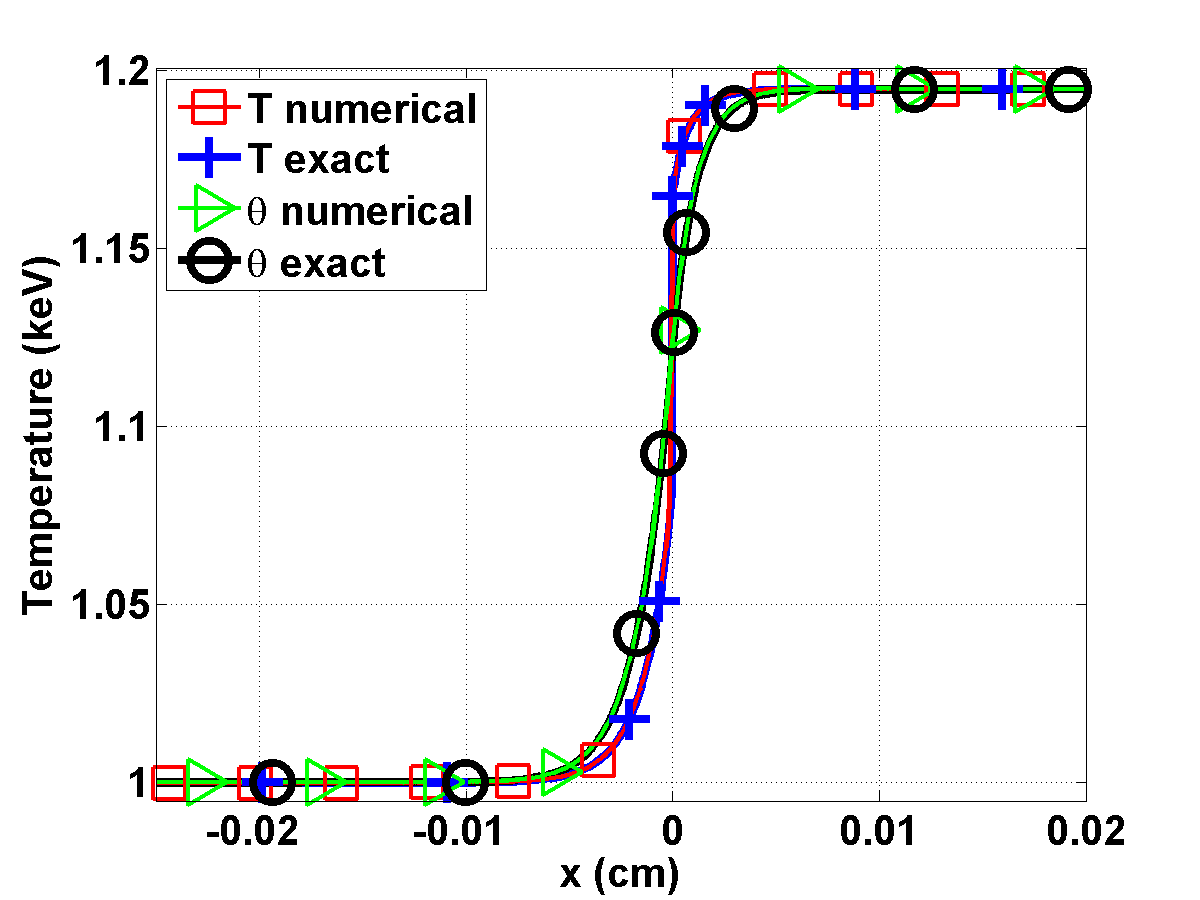
\includegraphics[width=\textwidth]{Mach_1p2_nel_1000_temperature.png}
        \caption{Material and radiation temperature profiles at steady-state for Mach 1.2 test.}\label{fig:Mach12_temp}
\end{figure}
The radiation and material temperatures have two different behaviors (\fig{fig:Mach12_temp}): the later experiences an embedded hydrodynamic shock, whereas the radiation temperature is smooth because of the diffusion term. The material temperature profile does not show any pre- and post-shock oscillations. In \fig{fig:Mach12_density}, the material density profile has a shock as well. The viscosity coefficient (\fig{fig:Mach12_viscosity}) is peaked in the shock as expected but does not saturate to the first-order viscosity. It is conjectured that the diffusion term in the radiation equation brings extra stability to the system. \\
%It also noted that pre- and post-shock oscillations occur in \fig{fig:Mach12_viscosity}, but do not affect the numerical solution because of their magnitude. \\
Overall, the numerical solution behaves as expected in the shock and the entropy-based viscosity method seems to efficiently smooth oscillations out.  
\begin{figure}[H]
                \centering
                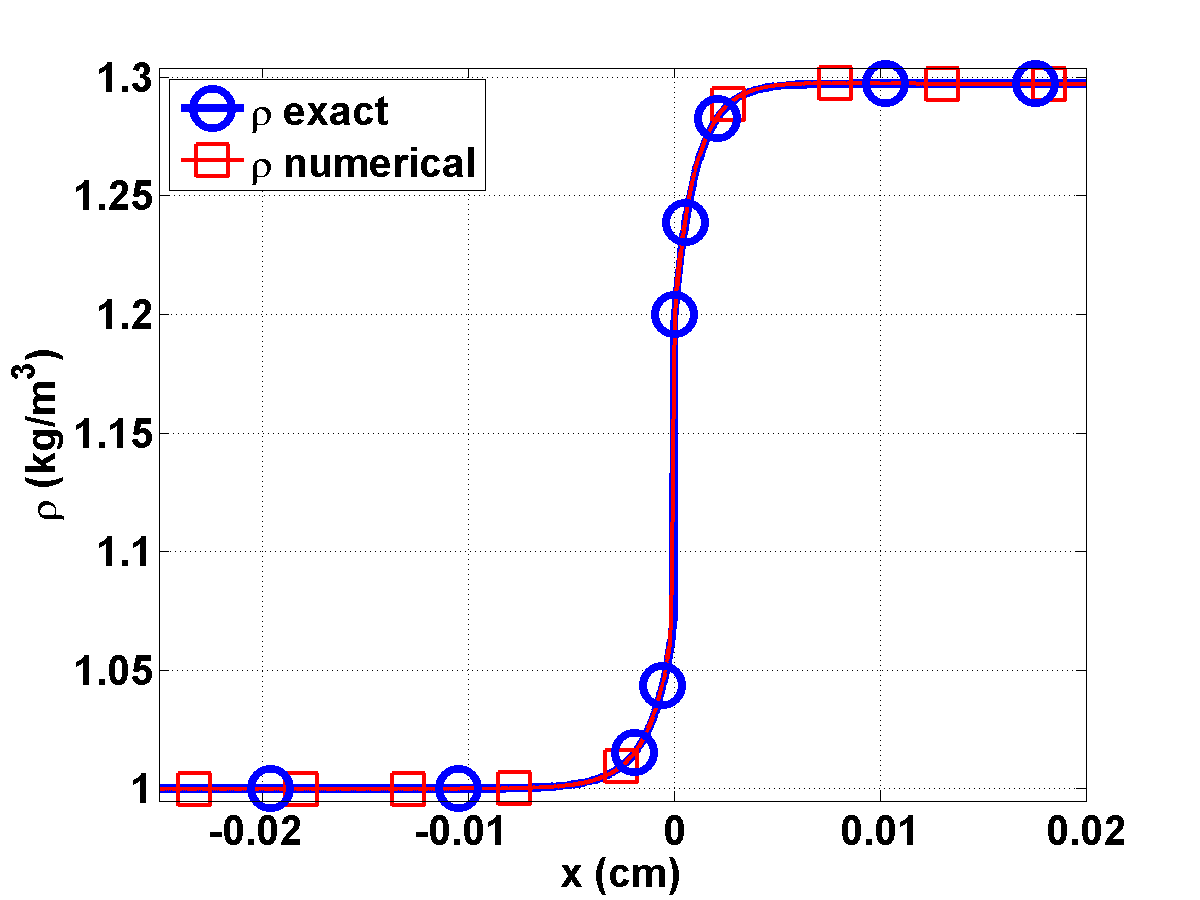
\includegraphics[width=\textwidth]{Mach_1p2_nel_1000_density.png}
        \caption{Material density profile at steady-state for Mach 1.2 test.}\label{fig:Mach12_density}
\end{figure}
\begin{figure}[H]
                \centering
                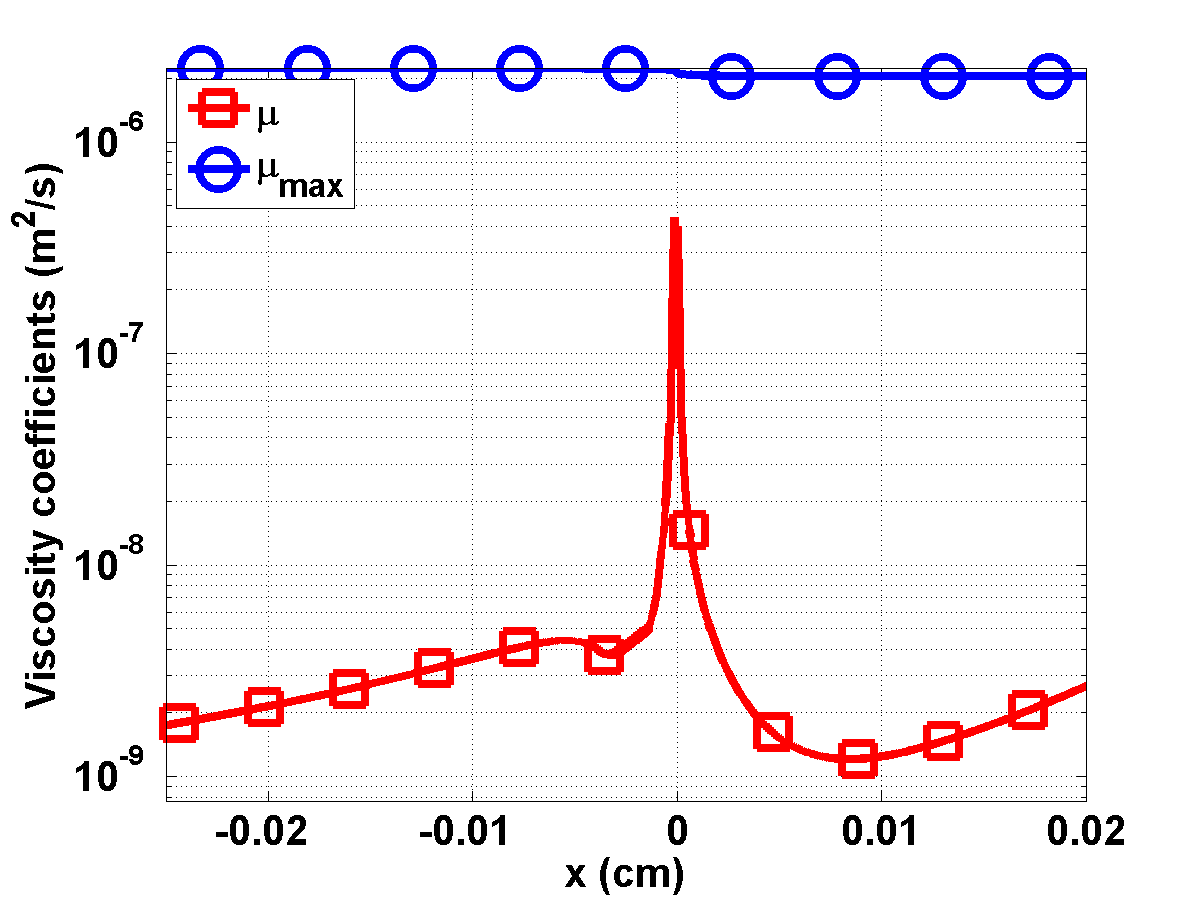
\includegraphics[width=\textwidth]{Mach_1p2_nel_1000_viscosity.png}
        \caption{First-order viscosity $\kappa_{max}$ and second-order viscosity $\kappa$ profiles at steady-state for Mach 1.2 test (logarithm scale).}\label{fig:Mach12_viscosity}
\end{figure}

\subsubsection{A Mach $2$ shock:}
%%%%%%%%%%%%%%%%%%%%%%%%%%%%%%%%%%%%%%%%%%%%%%%%%%%%%%%%%%%%%

The Mach $2$ shock test has two features: a hydrodynamic shock and a Zeldovich spike, which make it interesting for testing the robustness of the entropy-based viscosity method. The initial conditions are specified in \tbl{tbl:table5} for a slab of length $L=3 10^{-2}$ $cm$ with $x_0 = 0.$ $cm$.
\begin{table}[H]
\caption{\label{tbl:table5} Initial conditions for Mach $2$.}
\begin{center}
\begin{tabular}{|c|c|c|}
\hline 
 & left  & right \\ \hline
$\rho$ $(g/cm^3)$ &$1.$ & $1.0749588$ \\ \hline
$u$ $(cm/sh)$& $0.1405588$ & $0.1083456$ \\ \hline
$T$ $(keV)$& $0.1$ & $0.1194751$\\ \hline
$\epsilon$ $(jerks/cm^3)$ & $1.372$ $10^{-6}$ & $2.7955320$ $10^{-6}$\\
\hline
\end{tabular}  
\end{center}  
\end{table}
\begin{figure}[H]
                \centering
                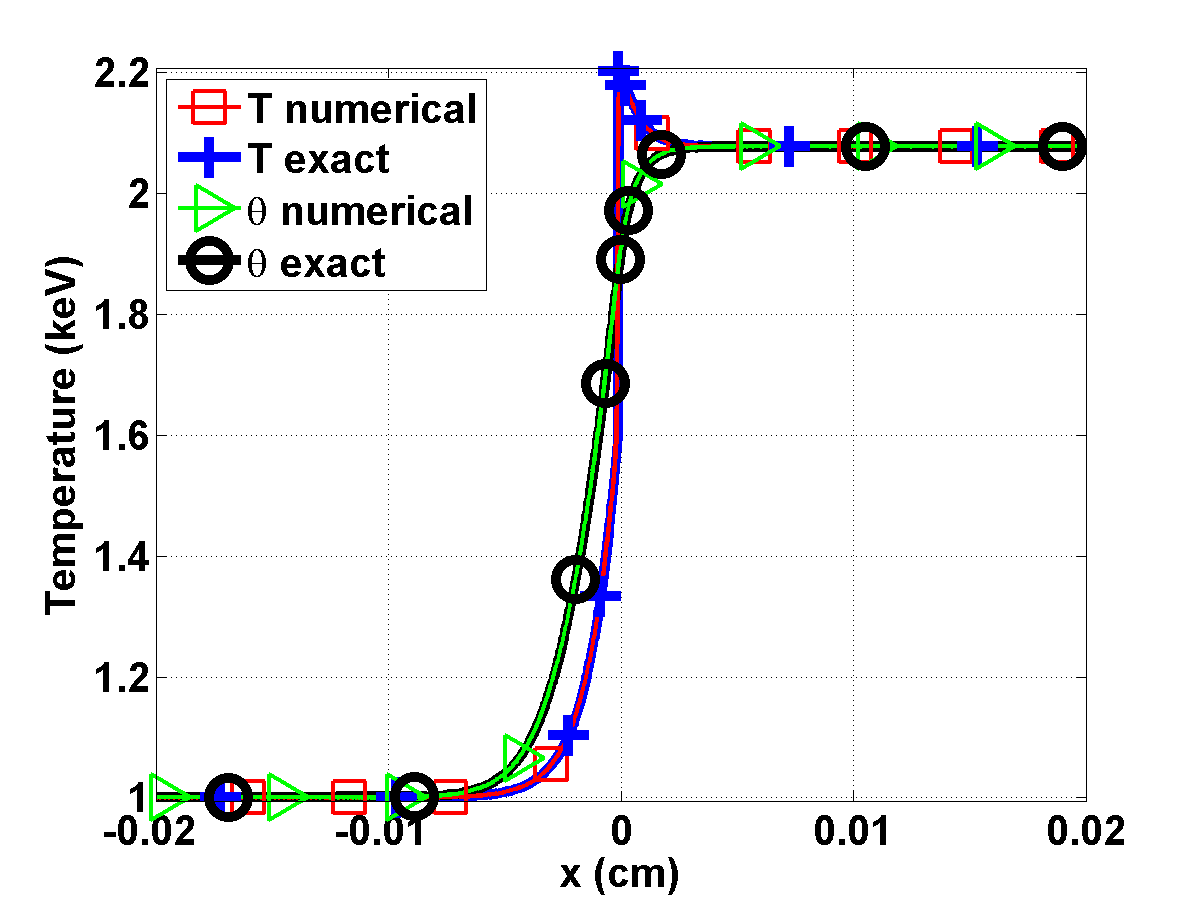
\includegraphics[width=\textwidth]{Mach_2_nel_2000_temperature.png}
        \caption{Material and radiation temperature profiles at steady-state for Mach 2 test.}\label{fig:Mach2_temp}
\end{figure}
Once again, the radiation temperature profile is smooth and the material temperature experiences an embedded hydrodynamic shock and a peak as shown in \fig{fig:Mach2_temp}. In \fig{fig:Mach2_density}, the shock is well resolved. The viscosity coefficient profile is given in \fig{fig:Mach2_viscosity} and is peaked, once again, in the shock region. \\
For academic purpose, the same simulation was run with the first-order viscosity i.e., $\kappa$ was set equal to $\kappa_{max}$ in the whole domain, in order to see the advantage of using a second-order viscosity coefficient. The results are given in \fig{fig:Mach2_tempEVandFO} for the material density and temperature. Numerical solutions with first- and second-order viscosity coefficients are graphed. The radiation temperature profile (not shown here) is not affected by the first-order viscosity and curves are confounded: this is expected because of the way the artificial viscosity term is treated in the radiation equation (\sect{sec:entropy-visc-meth}). However, on the same figure, the shock and peak in the material temperature profile are smoothed out: the shock is not as sharp and the peak amplitude is reduced because of the large amount of viscosity added to the system. This test shows the benefits of using a high-order viscosity coefficient in order to avoid over dissipation.
\begin{figure}[H]
                \centering
                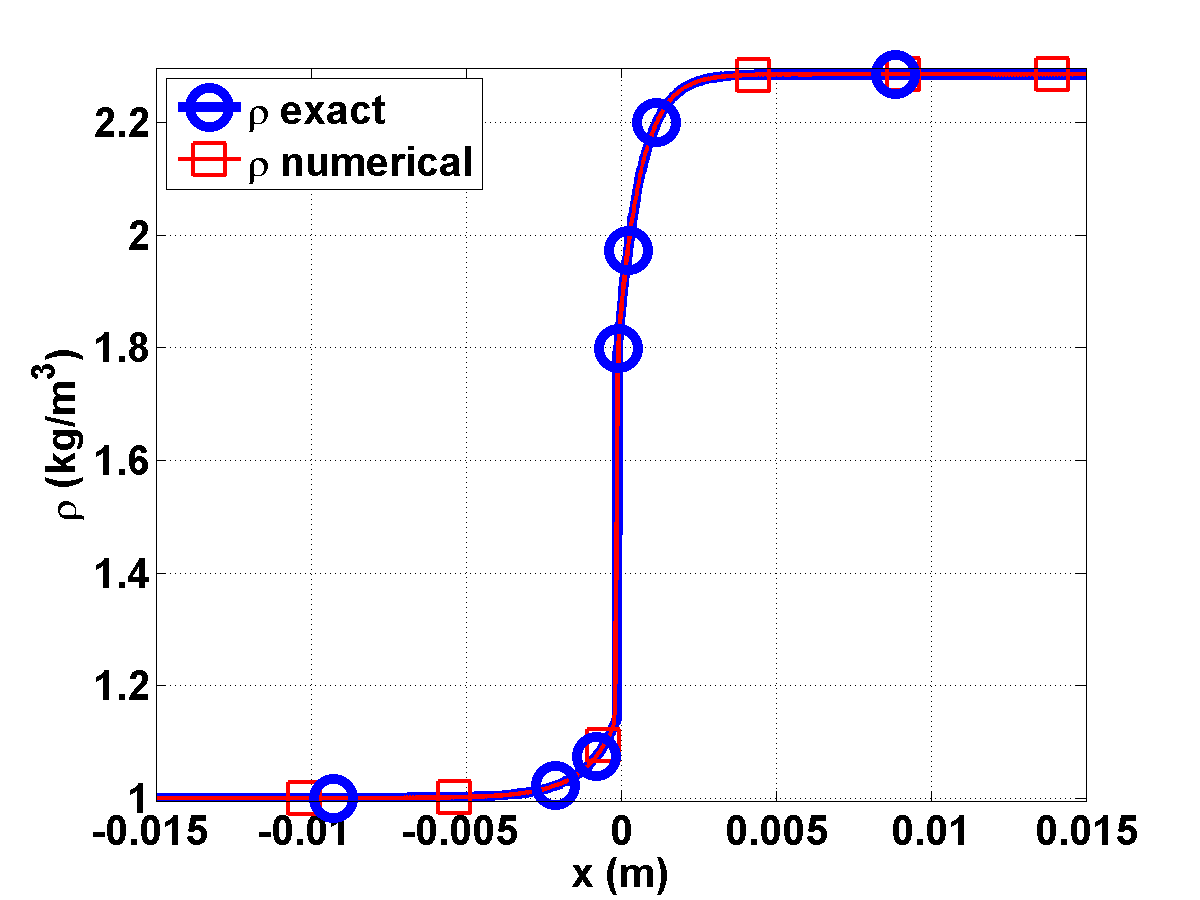
\includegraphics[width=\textwidth]{Mach_2_nel_2000_density.png}
        \caption{Material density profile at steady-state for Mach 2 test.}\label{fig:Mach2_density}
\end{figure}
\begin{figure}[H]
                \centering
                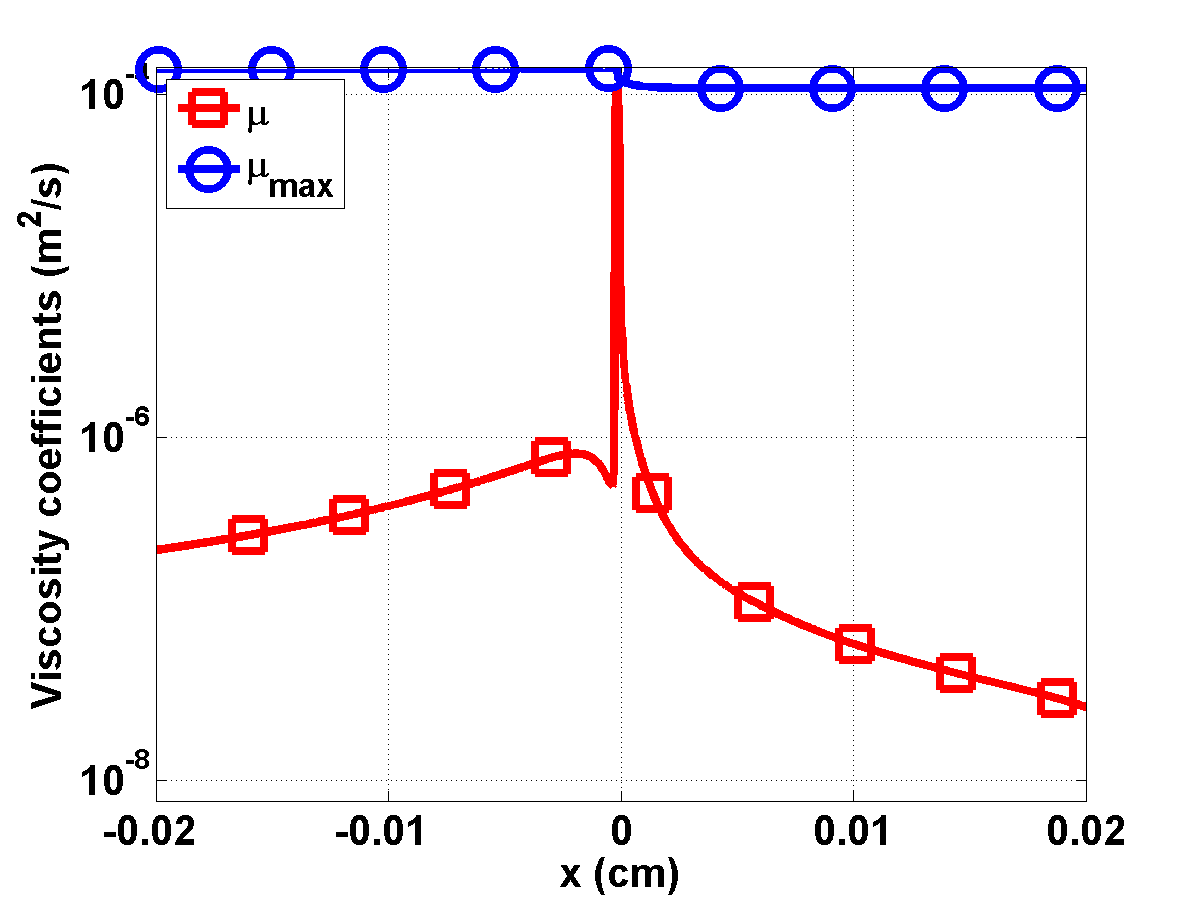
\includegraphics[width=\textwidth]{Mach_2_nel_2000_viscosity.png}
        \caption{First-order viscosity $\kappa_{max}$ and second-order viscosity $\kappa$ profiles at steady-state for Mach 2 test.}\label{fig:Mach2_viscosity}
\end{figure}
\begin{figure}[H]
                \centering
                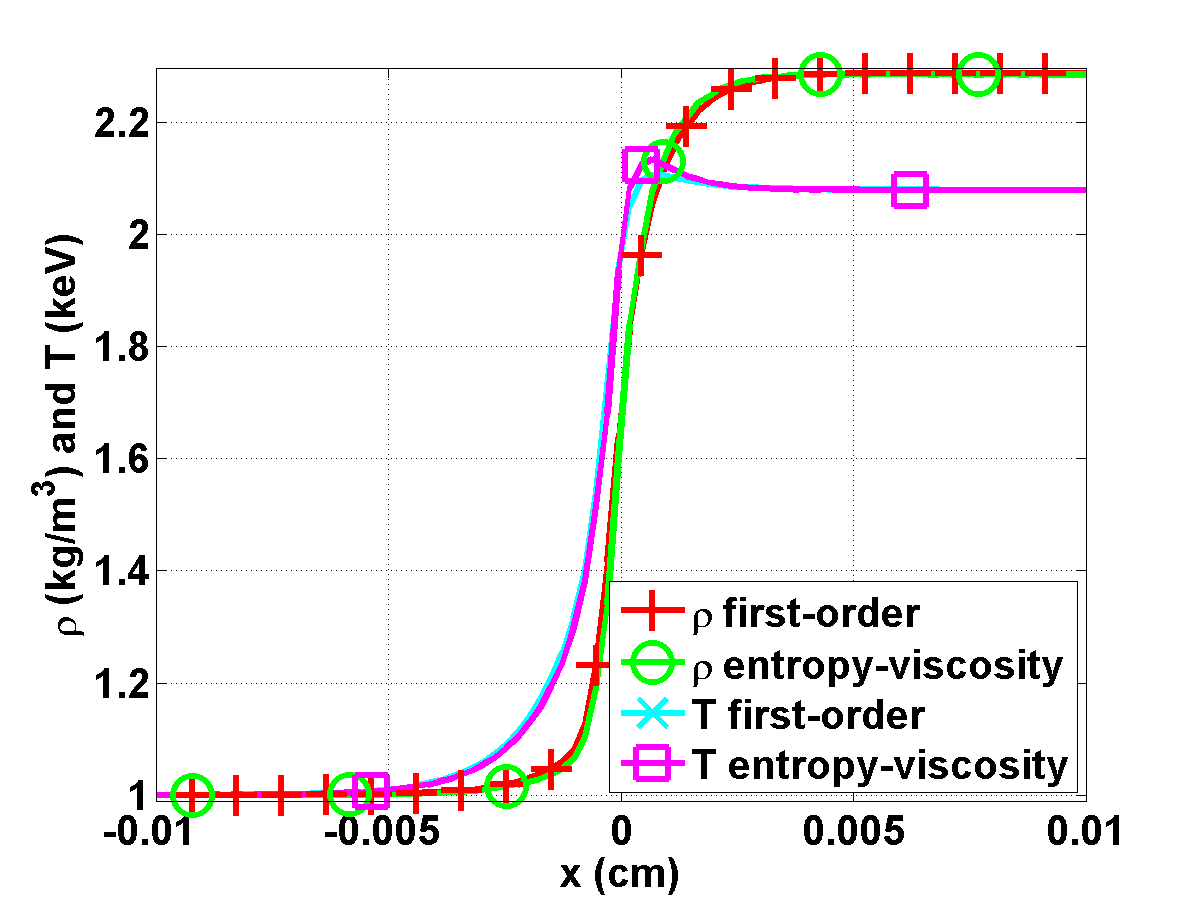
\includegraphics[width=\textwidth]{Mach_2_fo_ev.png}
        \caption{Comprarison between the material density and temperature profiles run with the high-order and first-order viscosity coefficients.}\label{fig:Mach2_tempEVandFO}
\end{figure}
%\begin{figure}[H]
 %               \centering
  %              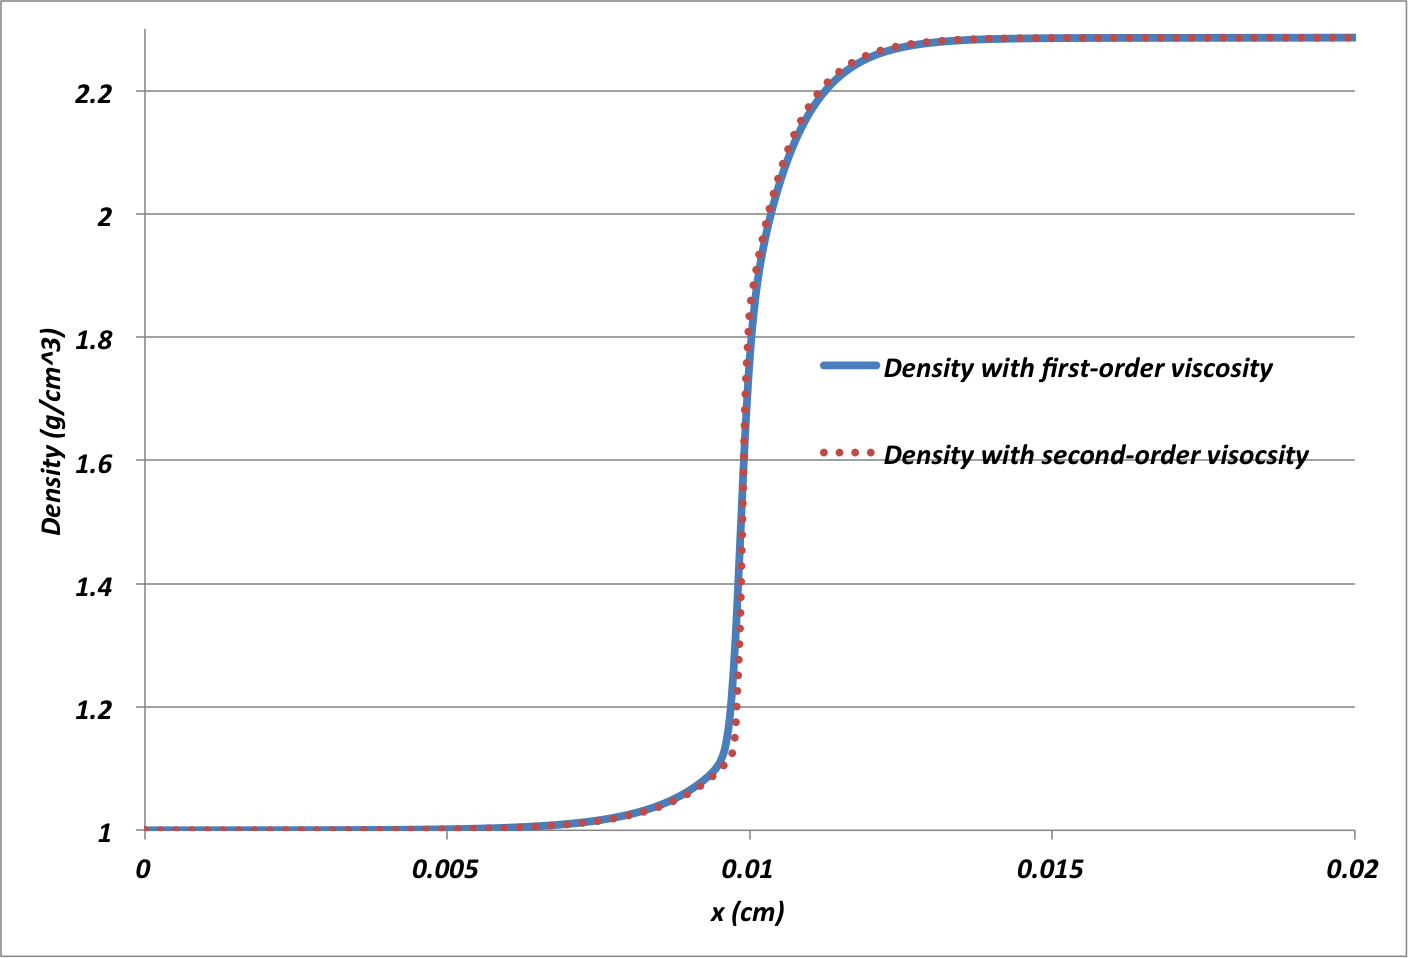
\includegraphics[width=\textwidth]{Mach2DensityEVandFO.png}
  %      \caption{Comparison between material density run with high-order and first-order viscosity: material density with second-order viscosity and material density with first-order viscosity.}\label{fig:Mach2_densityEVandFO}
%\end{figure}

\subsubsection{Mach $5$ shock:}
%%%%%%%%%%%%%%%%%%%%%%%%%%%%%%%%%%%%%%%%%%%%%%%%%%%%%%%%%%%%%
A Mach $5$ test is run with the initial conditions of \tbl{tbl:table6} on a computational domain of length $L=0.05$ $cm$ and with a $CFL$ of $10$ ($x_0 = 0$ $cm$). Steady-state results are shown in \fig{fig:Mach5_temp}, \fig{fig:Mach5_density} and \fig{fig:Mach5_viscosity} for the material and radiation temperatures, the density and the viscosity coefficients, respectively.
\begin{table}[H]
\caption{\label{tbl:table6} Initial conditions for Mach $5$.}
\begin{center}
\begin{tabular}{|c|c|c|}
\hline 
 & left  & right \\ \hline
$\rho$ $(g/cm^3)$ &$1.$ & $1.0749588$ \\ \hline
$u$ $(cm/sh)$& $0.1405588$ & $0.1083456$ \\ \hline
$T$ $(keV)$& $0.1$ & $0.1194751$\\ \hline
$\epsilon$ $(jerks/cm^3)$ & $1.372$ $10^{-6}$ & $2.7955320$ $10^{-6}$\\
\hline
\end{tabular}  
\end{center}  
\end{table}
\begin{figure}[H]
                \centering
                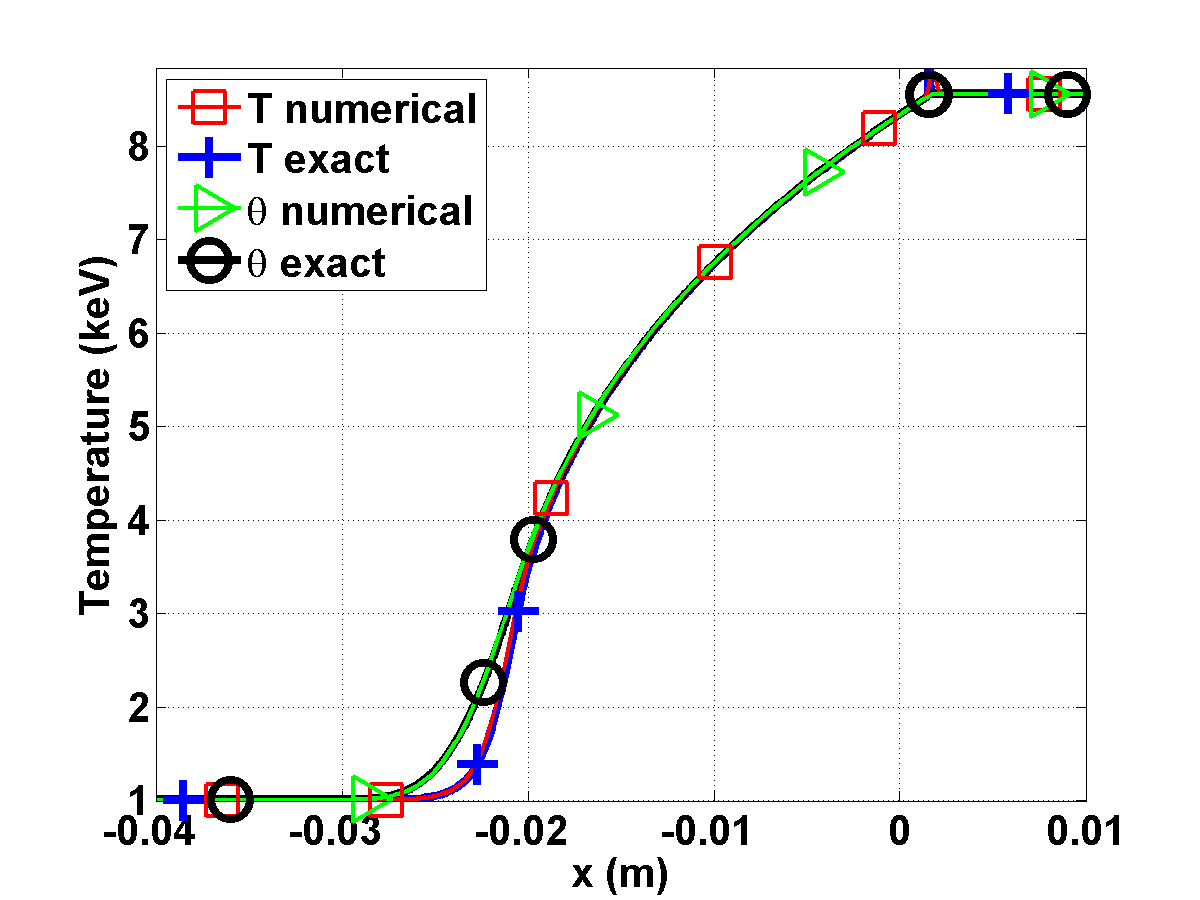
\includegraphics[width=\textwidth]{Mach_5_nel_1000_temperature.png}
        \caption{Material and radiation temperature profiles at steady-state for Mach 5 test. Zoom at the location go the peak using different mesh resolutions.}\label{fig:Mach5_temp}
\end{figure}
\begin{figure}[H]
                \centering
                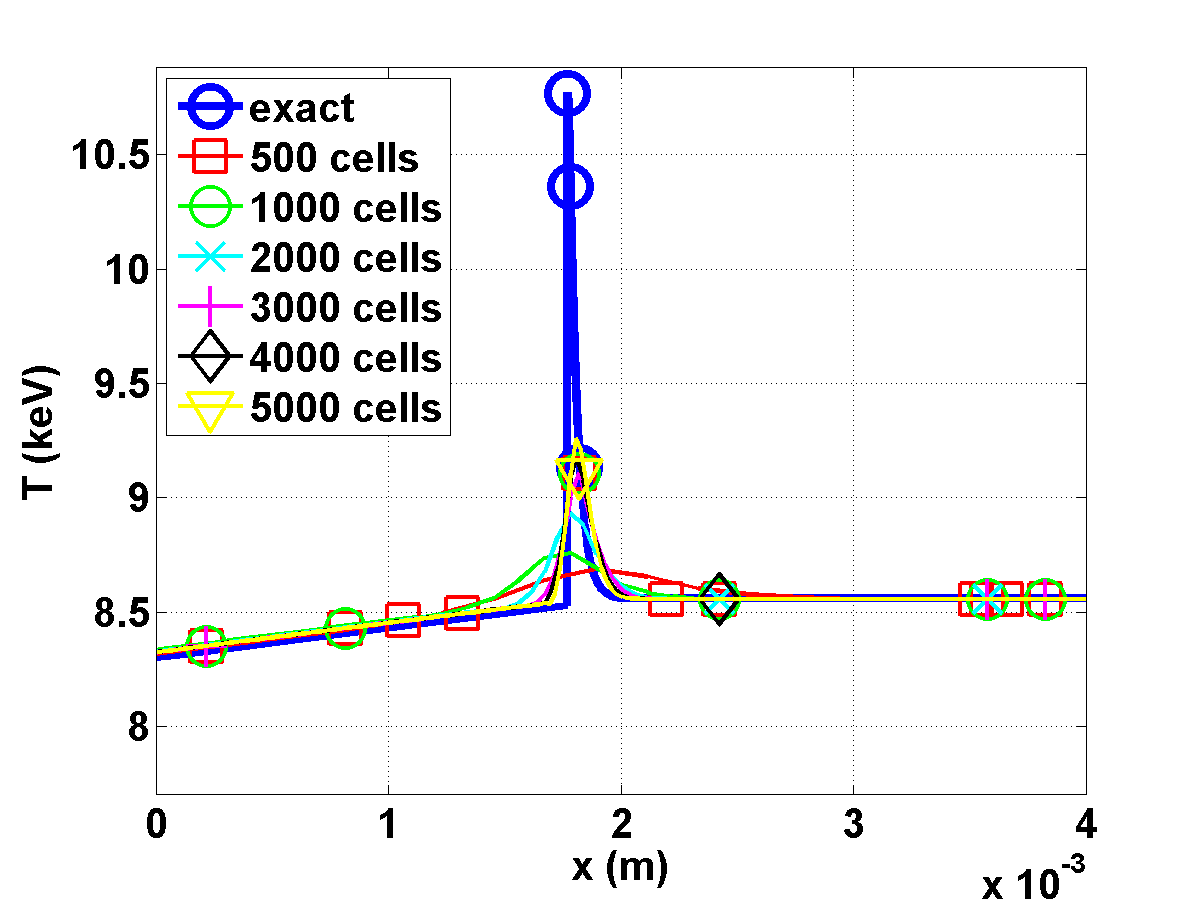
\includegraphics[width=\textwidth]{Mach_5_comparison.png}
        \caption{Material and radiation temperature profiles at steady-state for Mach 5 test. Zoom at the location go the peak using different mesh resolutions.}\label{fig:Mach5_comparison}
\end{figure}
In \fig{fig:Mach5_temp}, the radiation temperature profile is smooth. The material temperature no longer displayed an embedded hydrodynamic shock but has a Zeldovich spike. The mesh with $500$ elements is not fine enough to correctly resolve the Zeldovich spike. In \fig{fig:Mach5_comparison}, the Zeldovich spike region is plotted for different mesh from $500$ to $5000$ elements: the peak is better resolved when using large numbers of elements and its position seems to be independent of the mesh size when correctly refined. The density profile, \fig{fig:Mach5_density}, has a shock located at the same position as the Zeldovich spike of the material temperature profile. The viscosity coefficient $\kappa$ is also peaked in the shock region, as expected. The material and radiation variables do not present any oscillations. 
\begin{figure}[H]
                \centering
                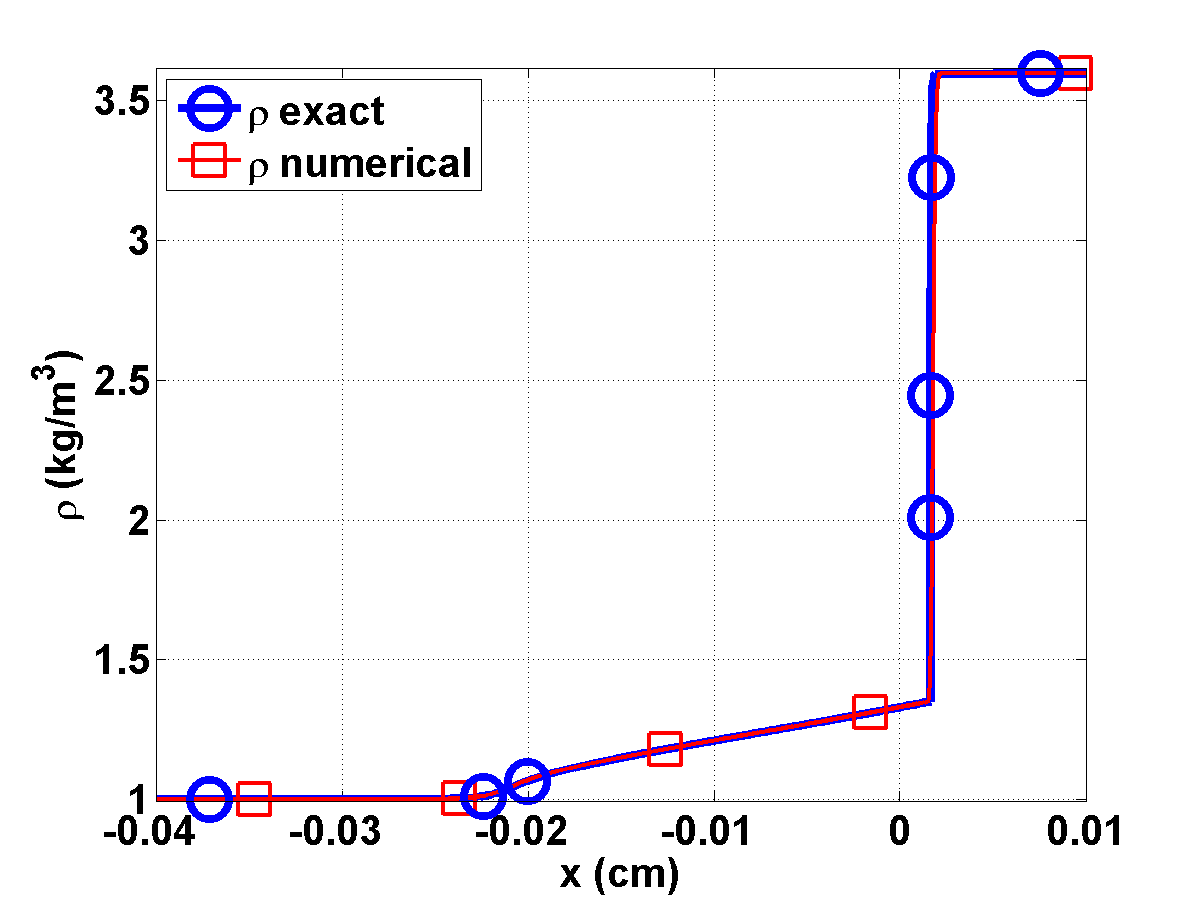
\includegraphics[width=\textwidth]{Mach_5_nel_2000_density.png}
        \caption{Material density profile at steady-state for Mach 5 test.}\label{fig:Mach5_density}
\end{figure}
\begin{figure}[H]
                \centering
                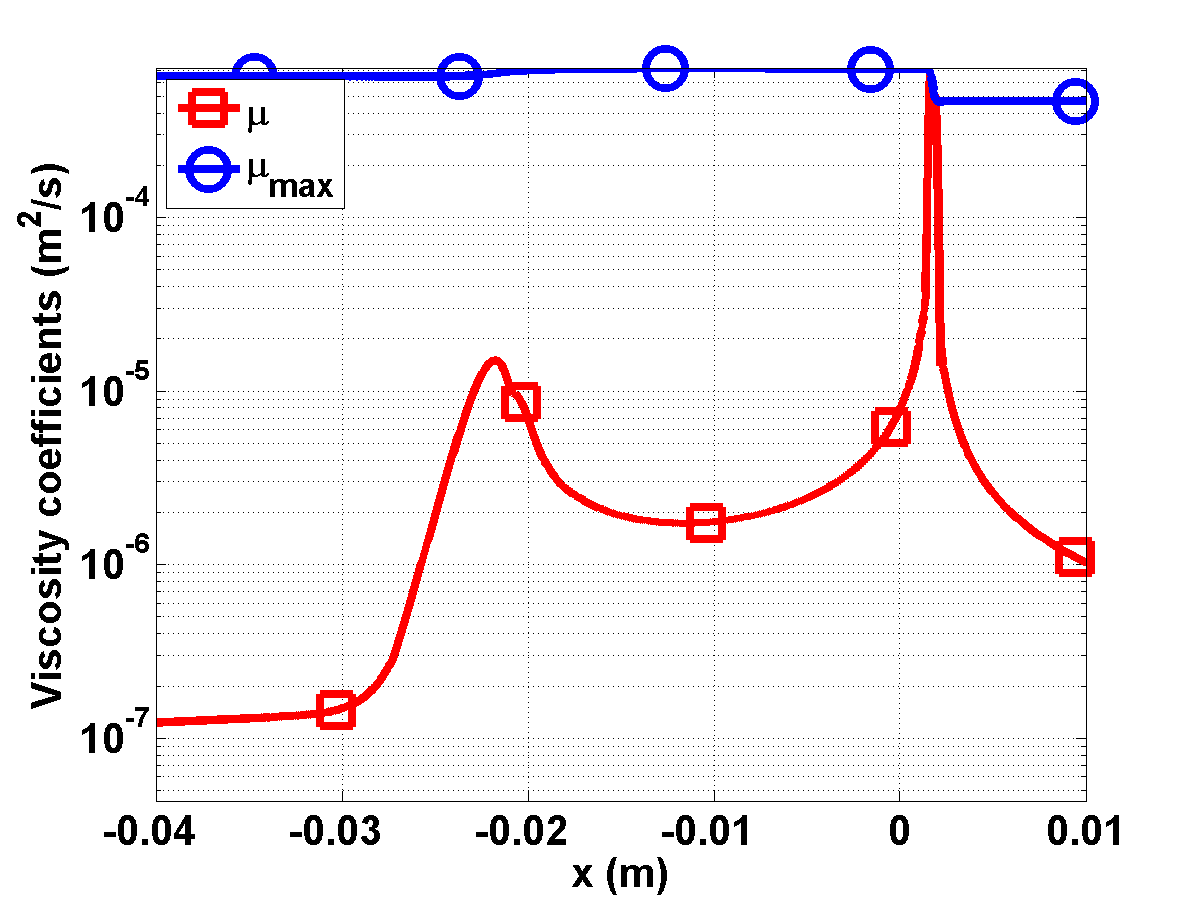
\includegraphics[width=\textwidth]{Mach_5_nel_2000_viscosity.png}
        \caption{First-order viscosity $\kappa_{max}$ and second-order viscosity $\kappa$ profiles at steady-state for Mach 5 test.}\label{fig:Mach5_viscosity}
\end{figure}

\subsubsection{Mach $50$ shock:} 
%%%%%%%%%%%%%%%%%%%%%%%%%%%%%%%%%%%%%%%%%%%%%%%%%%%%%%%%%%%%%

Mach $50$ test is known to be challenging. The initial conditions are given in \tbl{tbl:table7}. The computational domain is of length $L=0.2$ $cm$. Results are once again given at steady-state.
\begin{table}[H]
\caption{\label{tbl:table7} Initial conditions for Mach $50$.}
\begin{center}
\begin{tabular}{|c|c|c|}
\hline 
 & left  & right \\ \hline
$\rho$ $(g/cm^3)$ &$1.$ & $6.5189217$ \\ \hline
$u$ $(cm/sh)$& $585.6620$ & $89.84031$ \\ \hline
$T$ $(keV)$& $1.0$ & $85.51552$\\ \hline
$\epsilon$ $(jerks/cm^3)$ & $1.372$ $10^{-2}$ & $7.33726$ $10^{5}$\\
\hline
\end{tabular}  
\end{center}  
\end{table}
\begin{figure}[H]
                \centering
                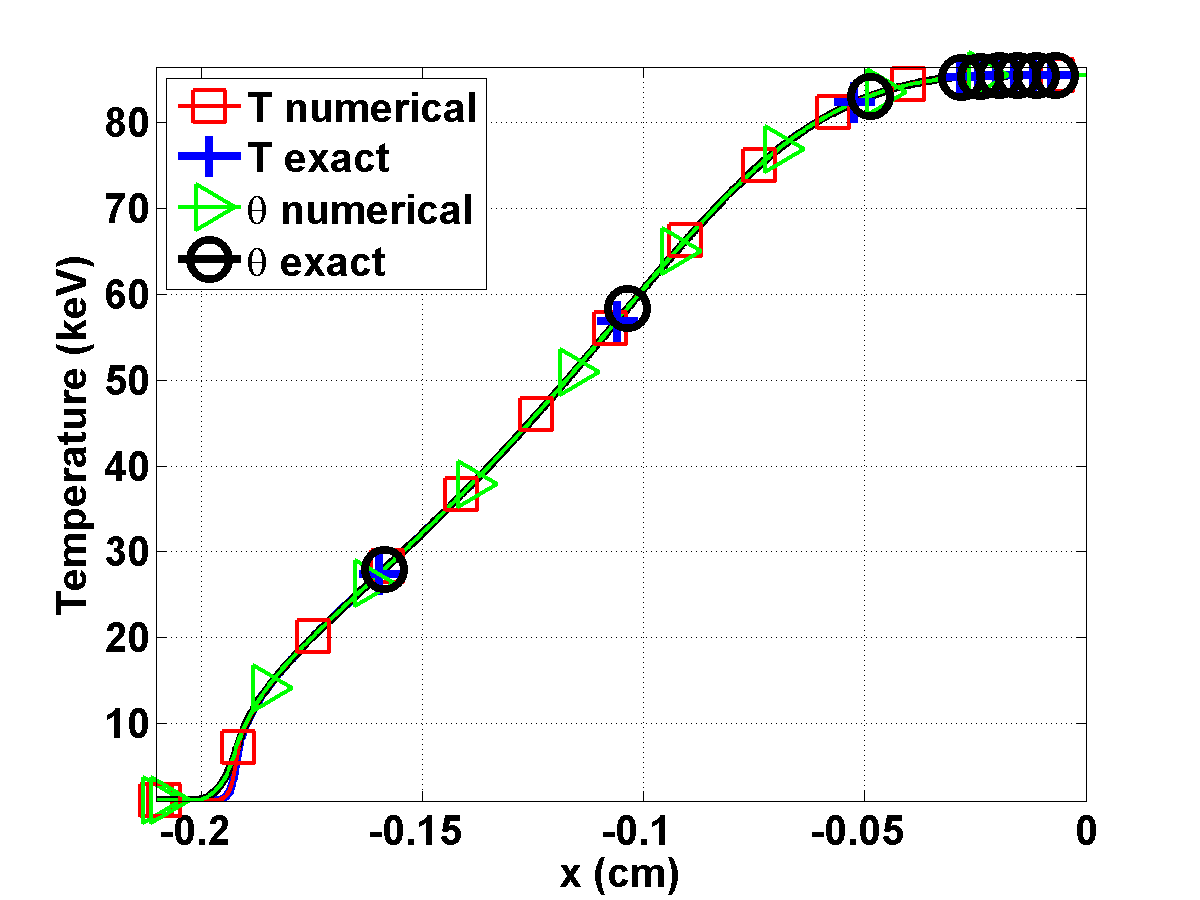
\includegraphics[width=\textwidth]{Mach_50_nel_1000_temperature.png}
        \caption{Material and radiation temperature profiles at steady-state for Mach 50 test.}\label{fig:Mach50_temp}
\end{figure}
At Mach $50$, there is no embedded hydrodynamic shock forming. The density profile is smooth as shown in \fig{fig:Mach50_density}. In \fig{fig:Mach50_temp}, the material and radiation temperatures overlap on all of the computational domain except for a small region located between $x=-0.2$ and $x=-0.18$ $cm$. In this particular region, the viscosity coefficient saturates to the first-order viscosity (\fig{fig:Mach50_viscosity}) because of the inflection point in the material temperature profile. The artificial dissipative terms correctly stabilize the material temperature profile without altering the physical solution: the radiation temperature is expected to increase ahead of the material temperature.
\begin{figure}[H]
                \centering
                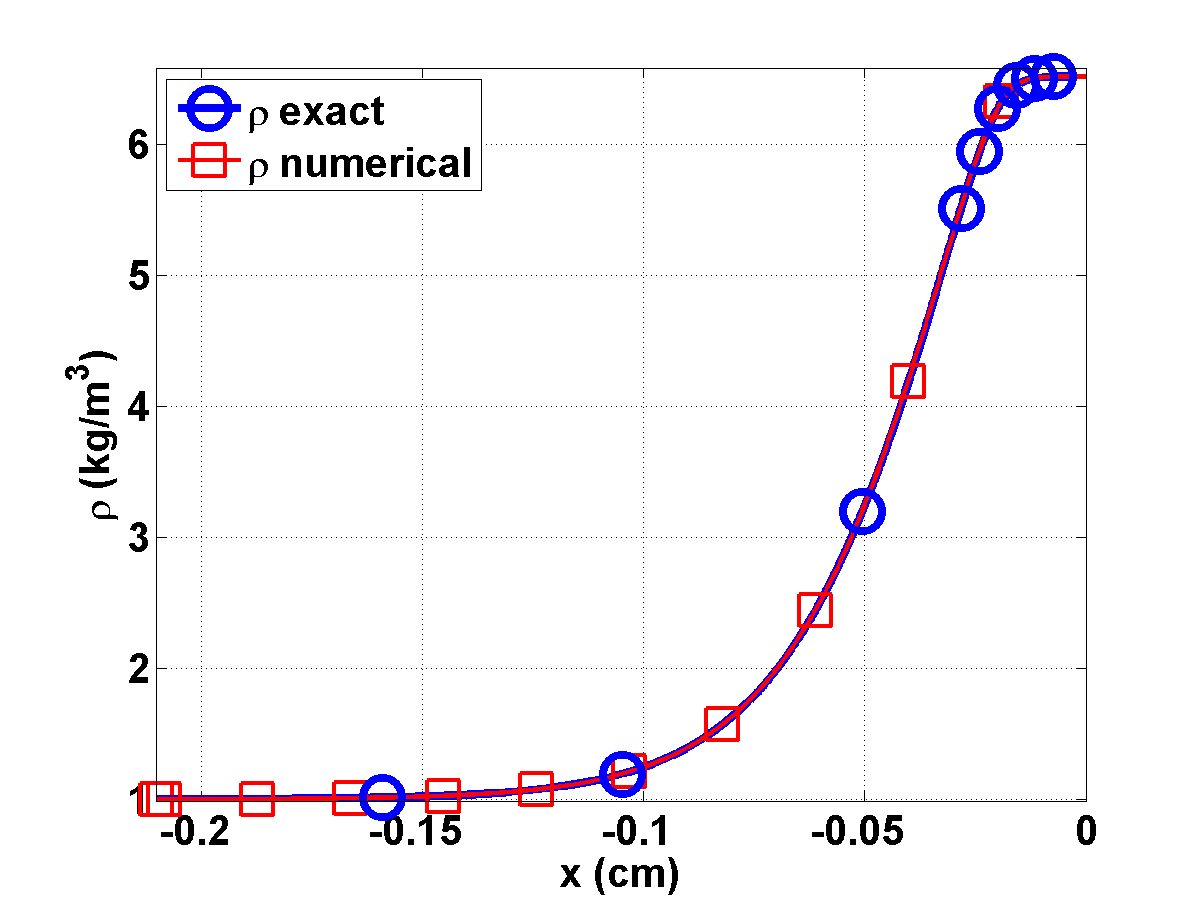
\includegraphics[width=\textwidth]{Mach_50_nel_1000_density.png}
        \caption{Material density profile at steady-state for Mach 50 test.}\label{fig:Mach50_density}
\end{figure}
\begin{figure}[H]
                \centering
                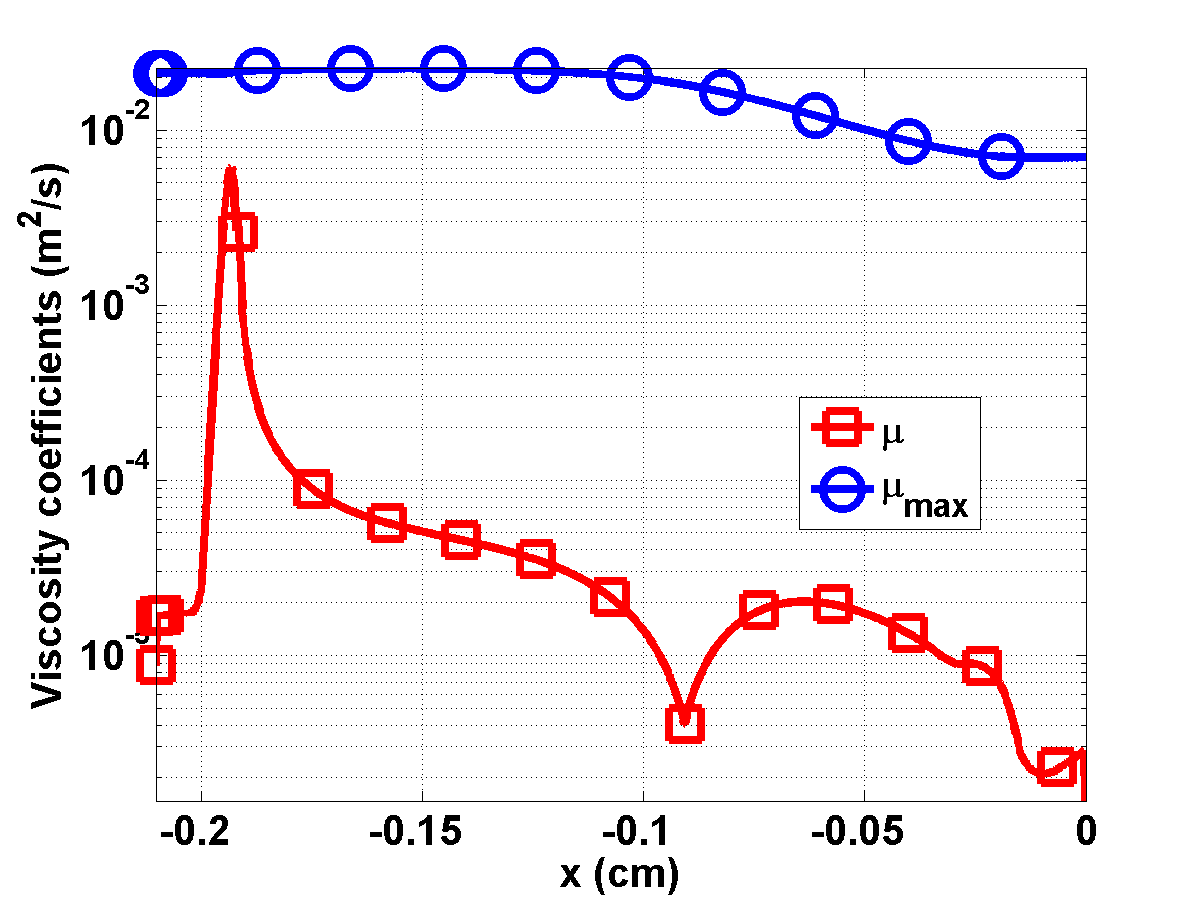
\includegraphics[width=\textwidth]{Mach_50_nel_1000_viscosity.png}
        \caption{First-order viscosity $\kappa_{max}$ and second-order viscosity $\kappa$ profiles at steady-state for Mach 50 test.}\label{fig:Mach50_viscosity}
\end{figure}

%%%%%%%%%%%%%%%%%%%%%%%%%%%%%%%%%%%%%%%%%%%%%%%%%%%%%%%%%%%%%
%%%%%%%%%%%%%%%%%%%%%%%%%%%%%%%%%%%%%%%%%%%%%%%%%%%%%%%%%%%%%
\section{Conclusions}
%%%%%%%%%%%%%%%%%%%%%%%%%%%%%%%%%%%%%%%%%%%%%%%%%%%%%%%%%%%%%
%%%%%%%%%%%%%%%%%%%%%%%%%%%%%%%%%%%%%%%%%%%%%%%%%%%%%%%%%%%%%
\label{sec:ccl}
In this paper, we have shown that the entropy-based viscosity method is a valid candidate for solving the $1$-D radiation-hydrodynamic equations. A theoretical derivation is given for the derivation of the dissipative terms that are consistent with the entropy minimum principle. The viscosity coefficient $\kappa$ is defined proportional to the entropy residual that measures the local entropy production allowing detection of shocks. Through the manufactured solution method, it is demonstrated, firstly, that second-order accuracy is achieved when the solution is smooth, and secondly, that the artificial dissipative terms do not affect the physical solution in the equilibrium-diffusion limit. \\
The method behaves well in the tests performed for Mach numbers ranging from $1.05$ to $50$. The main features such as the embedded hydrodynamic shock and the Zeldovich peak are resolved accurately without spurious oscillations. The viscosity coefficient is peaked in the shock region only and behaves as expected. All of these results were obtained by using an unique definition of the viscosity coefficient, that is computed on the fly. The addition of dissipative terms to the set of equations, requires more computational work but is rather simple to implement.\\
As future work, extension to the multi-D equations could be considered: all of the derivations presented in this paper hold. The definition of the viscosity coefficients $\kappa$ and $\kappa_{max}$ do not need to be modified.

%%%%%%%%%%%%%%%%%%%%%%%%%%%%%%%%%%%%%%%%%%%%%%%%%%%%%%%%%%%%%
\newpage
\begin{appendices}

%%%%%%%%%%%%%%%%%%%%%%%%%%%%%%%%%%%%%%%%%%%%%%%%%%%%%%%%%%%%%
%%%%%%%%%%%%%%%%%%%%%%%%%%%%%%%%%%%%%%%%%%%%%%%%%%%%%%%%%%%%%
\section{Proof of the entropy minimum principle for the radiation-hydrodynamic equations with dissipative terms:}
\label{app:appendixA}
%%%%%%%%%%%%%%%%%%%%%%%%%%%%%%%%%%%%%%%%%%%%%%%%%%%%%%%%%%%%%
%%%%%%%%%%%%%%%%%%%%%%%%%%%%%%%%%%%%%%%%%%%%%%%%%%%%%%%%%%%%%
In this appendix, a demonstration of the entropy minimum principle for the system of equations \eqt{eq:equation7} is given. This proof, inspired by \cite{jlg}, details the steps that lead to the derivation of the dissipative terms for the multi-D Euler equations by using the entropy minimum principle.\\
We start with the hyperbolic system given in \eqt{eq:equation3} and add dissipative terms to each equation as follows:
\begin{equation}
\label{eq:app_equ1bis}
\left\{
\begin{array}{llll}
\frac{d \rho}{dt} + \rho \partial_x u = \partial_x f \\
\partial_t (\rho u) + \partial_x \left(\rho u^2 +  P + \frac{\epsilon}{3} \right) = \partial_x g  \\
\partial_t (\rho E) + \partial_x \left[ u \left( \rho E +P \right) \right] = \partial_x \left( h + ug \right) \\
\partial_t \epsilon + u \partial_x \epsilon + \frac{4}{3} \epsilon \partial_x u = \partial_x l
\end{array}
\right.
\end{equation}
where $f$, $g$, $h$ and $l$ are dissipative terms to be determined.
\eqt{eq:app_equ1bis} is then recast as a function of the primitive variables $(\rho, u, e, \epsilon)$ to yield:
\begin{equation}
\label{eq:app_equ1}
\left\{
\begin{array}{llll}
\frac{d \rho}{dt} + \rho \partial_x u = \partial_x f \\
\rho \frac{du}{dt} + \partial_x \left( P + \frac{\epsilon}{3} \right) = \partial_x g - u \partial_x f  \\
\rho \frac{de}{dt} + P \partial_x u = \partial_x h + g \partial_x u + \left( 0.5 u^2 - e \right) \partial_x f \\
\frac{d\epsilon}{dt} + \frac{4}{3} \epsilon \partial_x u = \partial_x l
\end{array}
\right.
\end{equation}
The right-hand side of the internal energy equation can be simplified by choosing the dissipative terms $g$ and $h$ as follows: $h = \tilde{h} -0.5 u^2 f$ and $g = \rho \mu \partial_x u + uf$ where $\mu \geq 0$ is a dissipative coefficient. Using these definitions, the system of equation given in \eqt{eq:app_equ1} becomes:
\begin{equation}
\label{eq:app_equ1ter}
\left\{
\begin{array}{llll}
\frac{d \rho}{dt} + \rho \partial_x u = \partial_x f \\
\rho \frac{du}{dt} + \partial_x \left( P + \frac{\epsilon}{3} \right) = \partial_x g - u \partial_x f  \\
\rho \frac{de}{dt} + P \partial_x u = \rho \mu (\partial_x u)^2 + \partial_x \tilde{h} - e \partial_x f \\
\frac{d\epsilon}{dt} + \frac{4}{3} \epsilon \partial_x u = \partial_x l
\end{array}
\right.
\end{equation}
This system of equation admits an entropy function $s$ that depends on density $\rho$, internal energy $e$ and radiation energy density $\epsilon$. In order to prove the entropy minimum principle, a conservation statement satisfied by the entropy is needed. This equation which is referred to as an entropy residual $D_e(x,t)$, can be obtained by a combination of the equations given in \eqt{eq:app_equ1ter}. This process is motivated by the following (chain rule) 
%\comment{I think you still had a mistake. Check my correction.\color{blue}{I do not see where the mistake is}}
\begin{equation}
\label{eq:app_equ2}
\partial_{\alpha} s = \partial_{\rho} s \partial_{\alpha} \rho +  \partial_{e} s \partial_{\alpha}e +  \partial_{\epsilon} s \partial_{\alpha} \epsilon \text{,}
\end{equation}
 which holds for any independent variable $\alpha=x,t$. It is also required to define the dissipative terms $\tilde{h}$, $f$ and $l$. The following definitions are chosen:
 \begin{equation}
 \left\{
 \begin{array}{ccc}
f &= \kappa \partial_x \rho \\
\tilde{h} &= \kappa \partial_x (\rho e) \\
l &= \kappa \partial_x \epsilon
 \end{array}
 \right.
 \end{equation}
 where $\kappa$ is another positive dissipative coefficient. \\
 Thus, using the continuity, the internal energy and the radiation equations of \eqt{eq:app_equ1ter} and using \eqt{eq:app_equ2} along with the definition of the dissipative terms, a conservation statement satisfied by the entropy $s$ is obtained:
 \begin{eqnarray}
 \label{eq:app_equ3}
 \frac{ds}{dt} + \underbrace{\left( P \partial_e s + \rho^2 \partial_{\rho} s + \frac{4}{3} \rho \epsilon \partial_{\epsilon} s \right) \partial_x u}_\textrm{(a)} = \partial_x \left( \rho \kappa \partial_x s \right) + \kappa \partial_e s \partial_x s - \rho \kappa \underbrace{X A X^t}_\textrm{(b)} + \underbrace{ s_e \rho \mu (\partial_x u)^2}_\textrm{(c)}
 \end{eqnarray}
 where $X$ is a row vector defined as $X=\left( \rho, e, \epsilon \right)$ and $A$ is the $3$x$3$ symmetric matrix:
 \begin{equation}
 A = 
 \left[
 \begin{array}{ccc}
\partial_{\rho} \left( \rho^2 \partial_{\rho} s \right) & \partial_{\rho,e} s & \partial_{\rho} \left( \rho \partial_{\epsilon} s \right) \\
 \partial_{\rho,e} s & \partial_{e,e} s & \partial_{e,\epsilon} s \\
 \partial_{\rho} \left( \rho \partial_{\epsilon} s \right) & \partial_{e,\epsilon} s & \partial_{\epsilon,\epsilon} s
 \end{array}
 \right]
 \end{equation}
 In order to show that an entropy minimum principle holds, the signs of the terms $(a)$, $(b)$ and $(c)$ in \eqt{eq:app_equ3} need to be studied.\\
Regarding $(a)$, it is assumed that $P \partial_e s + \rho^2 \partial_{\rho} s + \frac{4}{3} \rho \epsilon \partial_{\epsilon} s=0$. The motivation for this is two-fold: First, in order to have a negative sign for the term $(a)$, it would require $P \partial_e s + \rho^2 \partial_{\rho} s + \frac{4}{3} \rho \epsilon \partial_{\epsilon} s$ to have a sign of opposite to that $\partial_x u$. The thermodynamic variables cannot be a function of the material velocity or its derivative under a non-relativistic assumption. Such a statement would not be true when dealing with relativistic equations of state. Second, a similar assumption was made in \cite{jlg} for multi-D Euler equations (without the radiation energy): $P \partial_e s + \rho^2 \partial_{\rho} s = 0$.\\
The term $(b)$, $XAX^t$, is a quadratic form and its sign is determined by simply looking at the positiveness of the matrix $A$ \cite{Evans}. Here we need to prove that $A$ is negative-definite which is equivalent to showing the three following inequalities:
\begin{equation}
 \left\{
 \begin{array}{ccc}
 A_1 \geq 0 \\
 A_2 \leq 0 \\
 A_3 = A \geq 0
 \end{array}
 \right.
 \end{equation}
 where $A_k$ is the $k^{th}$ order leading principle minor. Determining the sign of the last inequality that corresponds to the determinant of the $3$ by $3$ matrix $A$ can be difficult and needs to be simplified. Zeroing out the off-diagonal entries of the last row or column would simplify the expression for the determinant of $A$. This can be achieved by assuming $\partial_{\rho}(\rho \partial_{\epsilon} s)$ and $\partial_{e, \epsilon} s$ are zero, which requires the following form for the entropy function:
\begin{equation}
\label{eq:app_equ4}
s(\rho, e, \epsilon) = \tilde{s}(\rho,e) + \frac{\rho_0}{\rho}\hat{s}(\epsilon) \text{. } 
\end{equation}
where $\tilde{s}$ and $\hat{s}$ are two functions whose properties will be provided later. The constant $\rho_0$ is used for a dimensionality purpose.
Next, using the expression of the entropy given in \eqt{eq:app_equ4}, matrix $A$ becomes:
 \begin{equation}
 A = 
 \left[
 \begin{array}{ccc}
\partial_{\rho} \left( \rho^2 \partial_{\rho} \tilde{s} \right) & \partial_{\rho,e} \tilde{s} & 0 \\
 \partial_{\rho,e} \tilde{s} & \partial_{e,e} \tilde{s} & 0 \\
 0 & 0 & \rho^{-1} \partial_{\epsilon,\epsilon} \hat{s}
 \end{array}
 \right] \nonumber
 \end{equation}
 Proving that the matrix $A$ is  negative-definite is now straightforward by inspecting the sign of the leading principal minors:
 \begin{equation}
 \label{eq:A_matrix}
 \left\{
 \begin{array}{lll}
 A_1 = \partial_{\rho} \left( \rho^2 \partial_{\rho} \tilde{s} \right) \leq 0 \\
 A_2 = \partial_{\rho} \left( \rho^2 \partial_{\rho} \tilde{s} \right) \partial_{e,e} \tilde{s} - \left( \partial_{\rho,e} \tilde{s} \right)^2 \geq 0\\
 A_3 =  \rho^{-1} \partial_{\epsilon,\epsilon} \hat{s} A_2 \leq 0
 \end{array}
 \right.
 \end{equation} 
This is easily achieved when assuming that the functions $-\tilde{s}$ and $-\hat{s}$ are convex. Thus, the sign of $(b)$ is now determined. \\
 %This result is very strong since $\tilde{s}$ corresponds to the same entropy function as the one described in \cite{jlg}.\\
Finally, it remains to determine the sign of the term $(c) = \partial_e s \rho \mu (\partial_x u)^2$. The density $\rho$ and the viscosity coefficient $\mu$ are both positive: the latest proof for positivity of the density can be found in \cite{jlg}. Then, only the sign of $\partial_e s$ remains unknown but it can be determined by studying $(a)$. It was assumed earlier in this appendix that $P \partial_e s + \rho^2 \partial_{\rho} s + \frac{4}{3} \rho \epsilon \partial_{\epsilon} s=0$. This equation is now recast and split into two equations using \eqt{eq:app_equ4}. Separation of variables yields:
 \begin{equation}
 P \partial_e \tilde{s} + \rho^2 \partial_{\rho} \tilde{s} = \alpha \text{ and } \hat{s} - \frac{4\epsilon}{3} \partial_{\epsilon} \hat{s} = \alpha \nonumber
 \end{equation}
 where $\alpha$ is a constant to determine. If one sets $\alpha=0$, then the two physics are decoupled, which allows us to reconnect to the result derived in \cite{jlg} for the multi-D Euler equations: $P \partial_e \tilde{s} + \rho^2 \partial_{\rho} \tilde{s} = 0$. Then, following \cite{jlg}, definitions for $\partial_e \tilde{s}$ and $\partial_{\rho} \tilde{s}$ are obtained:
 \begin{equation}
 \label{eq:definition}
 \left\{
 \begin{array}{ll}
 \partial_e s = \partial_e \tilde{s} = T^{-1} \nonumber\\
 \partial_{\rho} \tilde{s} = -\frac{P}{\rho^2} \partial_e \tilde{s}
 \end{array}
 \right.
 \end{equation} 
 where $T$ is the material temperature which ensures positivity of $\partial_e s$. Thus, $(c)$ is positive. \\
From the above results, the entropy minimum principle follows, so that the sign of the entropy residual is known:
\begin{equation}
\boxed{\partial_t s + u \partial_x s \geq 0}
\end{equation}
 %%%%%%%%%%%%%%%
\begin{remark}
By assuming $\alpha=0$, an expression for the $\hat{s}$ can be derived by solving the ODE, $\hat{s} - \frac{4\epsilon}{3} \partial_{\epsilon} \hat{s} = 0$, which yields:
$\hat{s}(\epsilon) = \beta \exp \left(\frac{4 \epsilon^{2}}{3} \right)$, where $\beta$ is a constant. The sign of $\beta$ is determined by using the condition, $\partial_{\epsilon,\epsilon} \hat{s} \leq 0$, derived above, so that $\beta\leq0$.
\end{remark}
\begin{remark}
The viscous regularization derived in this appendix, has two viscosity coefficients: $\mu$ and $\kappa$. For the purpose of this paper, these coefficients are set equal. Under this assumption, the above viscous regularization is equivalent to the parabolic regularization of \cite{Parabolic}.
\end{remark}
\end{appendices}

%%%%%%%%%%%%%%%%%%%%%%%%%%%%%%%%%%%%%%%%%%%%%%%%%%%%%%%%%%%%%
%%%%%%%%%%%%%%%%%%%%%%%%%%%%%%%%%%%%%%%%%%%%%%%%%%%%%%%%%%%%%
\newpage
\addcontentsline{toc}{section}{Bibliography}
\begin{thebibliography}{24}

 \bibitem{Hussaini}
 \emph{Upwind and high-resolution schemes},
 Hussaini MY, van Leer B, Van Rosendale J, Berlin: Springer, 1997.
  
    \bibitem{jlg1}
  {\em Entropy viscosity method for nonlinear conservation laws}, 
  Jean-Luc Guermond, R. Pasquetti, B. Popov, J. Comput. Phys., 230 (2011) 4248-4267.
  
  \bibitem{jlg2}
  {\em Entropy Viscosity Method for High-Order Approximations of Conservation Laws}, 
  J-L. Guermond, R. Pasquetti, 
  Lecture Notes in Computational Science and Engineering, Springer, Volume 76, (2011) 411-418.

 \bibitem{Leveque}
 \emph{Numerical methods for conservation laws},
 LeVeque RJ, Lectures in Mathematics, Basel: Birhauser, 1990

  \bibitem{Balsara}
  \emph{An Analysis of the Hyperbolic Nature of the Equations of Radiation Hydrodynamics},
  Dinshaw S. Balsara, J. Quant. Spectrosc. Radiat. Transfer, Vol. 61, No. 5, pp. 617-627, 1999.
  
  \bibitem{LowrieMorelHittinger}
  \emph{Coupling radiation and hydrodynamics},
  Lowrie RB, Morel JE, Hittinger JA, 521 (1), 432-50 (1999).
  
  \bibitem{Woodward}
  \emph{Numerical simulations for radiation hydrodynamics. I. Diffusion limit}
  Dai W, Woodward PR, J. Comput Phys (1998), 142, 182-207.
  
  \bibitem{Wareing}
\emph{A diffusion synthetic acceleration method for the SN equations with discontinuous finite element space and time differencing},
T.A. Wareing, J.E. Morel, J.M. McGhee, Proceedings of the International COnference on Mathematics and Computation, Reactor Physics and Environmental Analysis in Nuclear Applications, Madrid, spain, September 27-30, vol. 1, pp. 45-44.
       
\bibitem{Hairer}
\emph{Solving ordinary differential equations II},
Second Revised ed., Springer Series in Computational Mathematics, Springer, New York, 2002.
 
 \bibitem{EdwardsMorelKnoll}
 \emph{Nonlinear variants of the TR$-$BDF$2$ method for thermal radiative diffusion},
 Jarrods D. Edwards, Jim E. Morel, Dana A. Knoll, Journal of Computational Physics, 230 (2011), 1198-1214.
 
\bibitem{Toro}
  \emph{Riemann Solvers and numerical methods for fluid dynamics.}
  E.F. Toro, $2^{nd}$ Edition, Springer.  
    
  \bibitem{valentin}
  \emph{Implementation of the entropy viscosity method with the discontinuous Galerkin method},
  Valentin Zingan, Jean-Luc Guermond, Jim Morel, Bojan Popov, Volume 253, 1 January 2013, Pages 479-490
  
 \bibitem{LowrieEdwards}
 \emph{Radiative shock solutions with grey non equilibrium diffusion},
 R. B. Lowrie, J. D. Edwards, Shock Waves (2008) 18:129-143.
 
 \bibitem{entropy}
 \emph{E. Tadmor. A minimum entropy principle in the gas dynamics equations},
  Appl. Numer. Math., 2(3-5):211�219, 1986.
    
  \bibitem{LowrieMorel}
  \emph{Issues with high-resolution Godunov methods for radiation hydrodynamics},
  R.B. Lowrie, J.E. Morel, Journal of Quantitative Spectroscopy \& Radiative Transfer, 69, 475-489 (2001).
  
\bibitem{Lax}
\emph{Weak solutions of nonlinear hyperbolic equations and their numerical computation},
P. Lax, Comm. Pure Appl. Math., 7:159-193, 1954.

\bibitem{Evans}
\emph{Numerical approximations of hyperbolic systems of conservation laws},
E. Godlewski and P.-A. Raviart, volume 118 of Applied Mathematical Sciences. Springer-Verlag, New York, 1996. ISBN 0-387-94529-6.

\bibitem{EdwardsMorelLowrie}
\emph{Second-Order Discretization in Space and Time for Radiation Hydrodynamics},
Jarrod D. Edwards, Jim E. Morel, Robert B. Lowrie, International Conference on Mathematics and Computational Methods Applied to Nuclear Science \& Engineering (M\&C 2013), Sun Valley, Idaho USA, May 5-9, American Nuclear Society, LaGrange Park, II (2013).
   
  \bibitem{ShiJin}
  \emph{Numerical Schemes for Hyperbolic Conservation Laws with Stiff Relaxation Terms}, 
  Shi Jin and C. David Levermore, Journal of Computational Physics, 126, 449-467 (1996).
  
  \bibitem{jlg}
  \emph{Viscous regularization of the Euler equations and entropy principles},
  Jean-Luc Guermond and Bojan Popov, under review.
  
  \bibitem{Moose}
  \emph{A parallel computational framework for coupled systems of nonlinear equations},
  D. Gaston, C. Newsman, G. Hansen and D. Lebrun-Grandie, Nucl. Eng. Design, vol 239, pp 1768-1778, 2009.
 
 \bibitem{JFNK}
 \emph{Jacobian-free Newton-Krylov methods: a survey of approaches and applications},
 Knoll D. A., Keyes D. E., Journal of Computational Physics, 193, 2, 357-397 (2004).
 
 \bibitem{SEM}
  \emph{The discrete equation method (DEM) for fully compressible, two-phase flows in ducts of spatially varying cross-section.}
  R.Berry, R.Saurel, O. LeMetayer,
  Nuclear Engineering and Design 240 (2010) 3797-3818.
  
  \bibitem{Parabolic}
  \emph{On positivity preserving finite volume schemes for Euler equations},
  Perthane B. and Shu C-W., Numer. Math., 73(1):119-130, 1996.
  
  \end{thebibliography}

%%%%%%%%%%%%%%%%%%%%%%%%%%%%%%%%%%%%%%%%%%%%%%%%%%%%%%%%%%%%%
%%%%%%%%%%%%%%%%%%%%%%%%%%%%%%%%%%%%%%%%%%%%%%%%%%%%%%%%%%%%%
\end{document}
